\newpage
    \subsection{Ekrany główne}
    Główną część aplikacji stanowi aktywność główna, w skład której wchodzą fragmenty obsługujące interakcję z mapą oraz zamieszonymi na niej miejscami.
    Nawigacja pomiędzy jego fragmentami następuje za pomocą dolnego paska nawigacyjnego należącego do biblioteki Material Design.

    \vspace{1cm}
        \subsubsection{Ekran mapy}
        Głównym ekranem, w którym użytkownik wykonuje najbardziej istotne akcje, jest ekran mapy. W nim widoczna jest, pobierana za pomocą Maps SDK for Android, mapa Google.
        Wygląd ekranu mapy zaprezentowany jest na rys.~\ref{map_fragment}. W prawym dolnym rogu mapy znajduje się przycisk centrujący ekran na pozycji użytkownika. Na górze 
        zlokalizowane są przyciski wyszukiwania miejsc. Przycisk opisany „Find new places!” (pol. Odkryj nowe miejsca) przeszukuje bazę danych w poszukiwaniu wszystkich miejsc 
        znajdujących się w promieniu trzystu metrów od środka ekranu. Przykład mapy z zaznaczonymi za pomocą przycisku „Find new places!” miejscami widoczny jest na rys.~\ref{find_places}.
        Na samej górze znajduje się grupa chipów opisanych nazwami kategorii. Przyciśnięcie chipa z napisem „shopping” (pol.\@ zakupy) jest analogiczne do przycisku „Find new places!”, ale pobrane
        zostaną tylko miejsca o kategorii „shopping”. 

        \vspace{1cm}
        \begin{figure}[H]%
            \centering
            \begin{subfigure}[b]{0.3\textwidth}
                \centering
                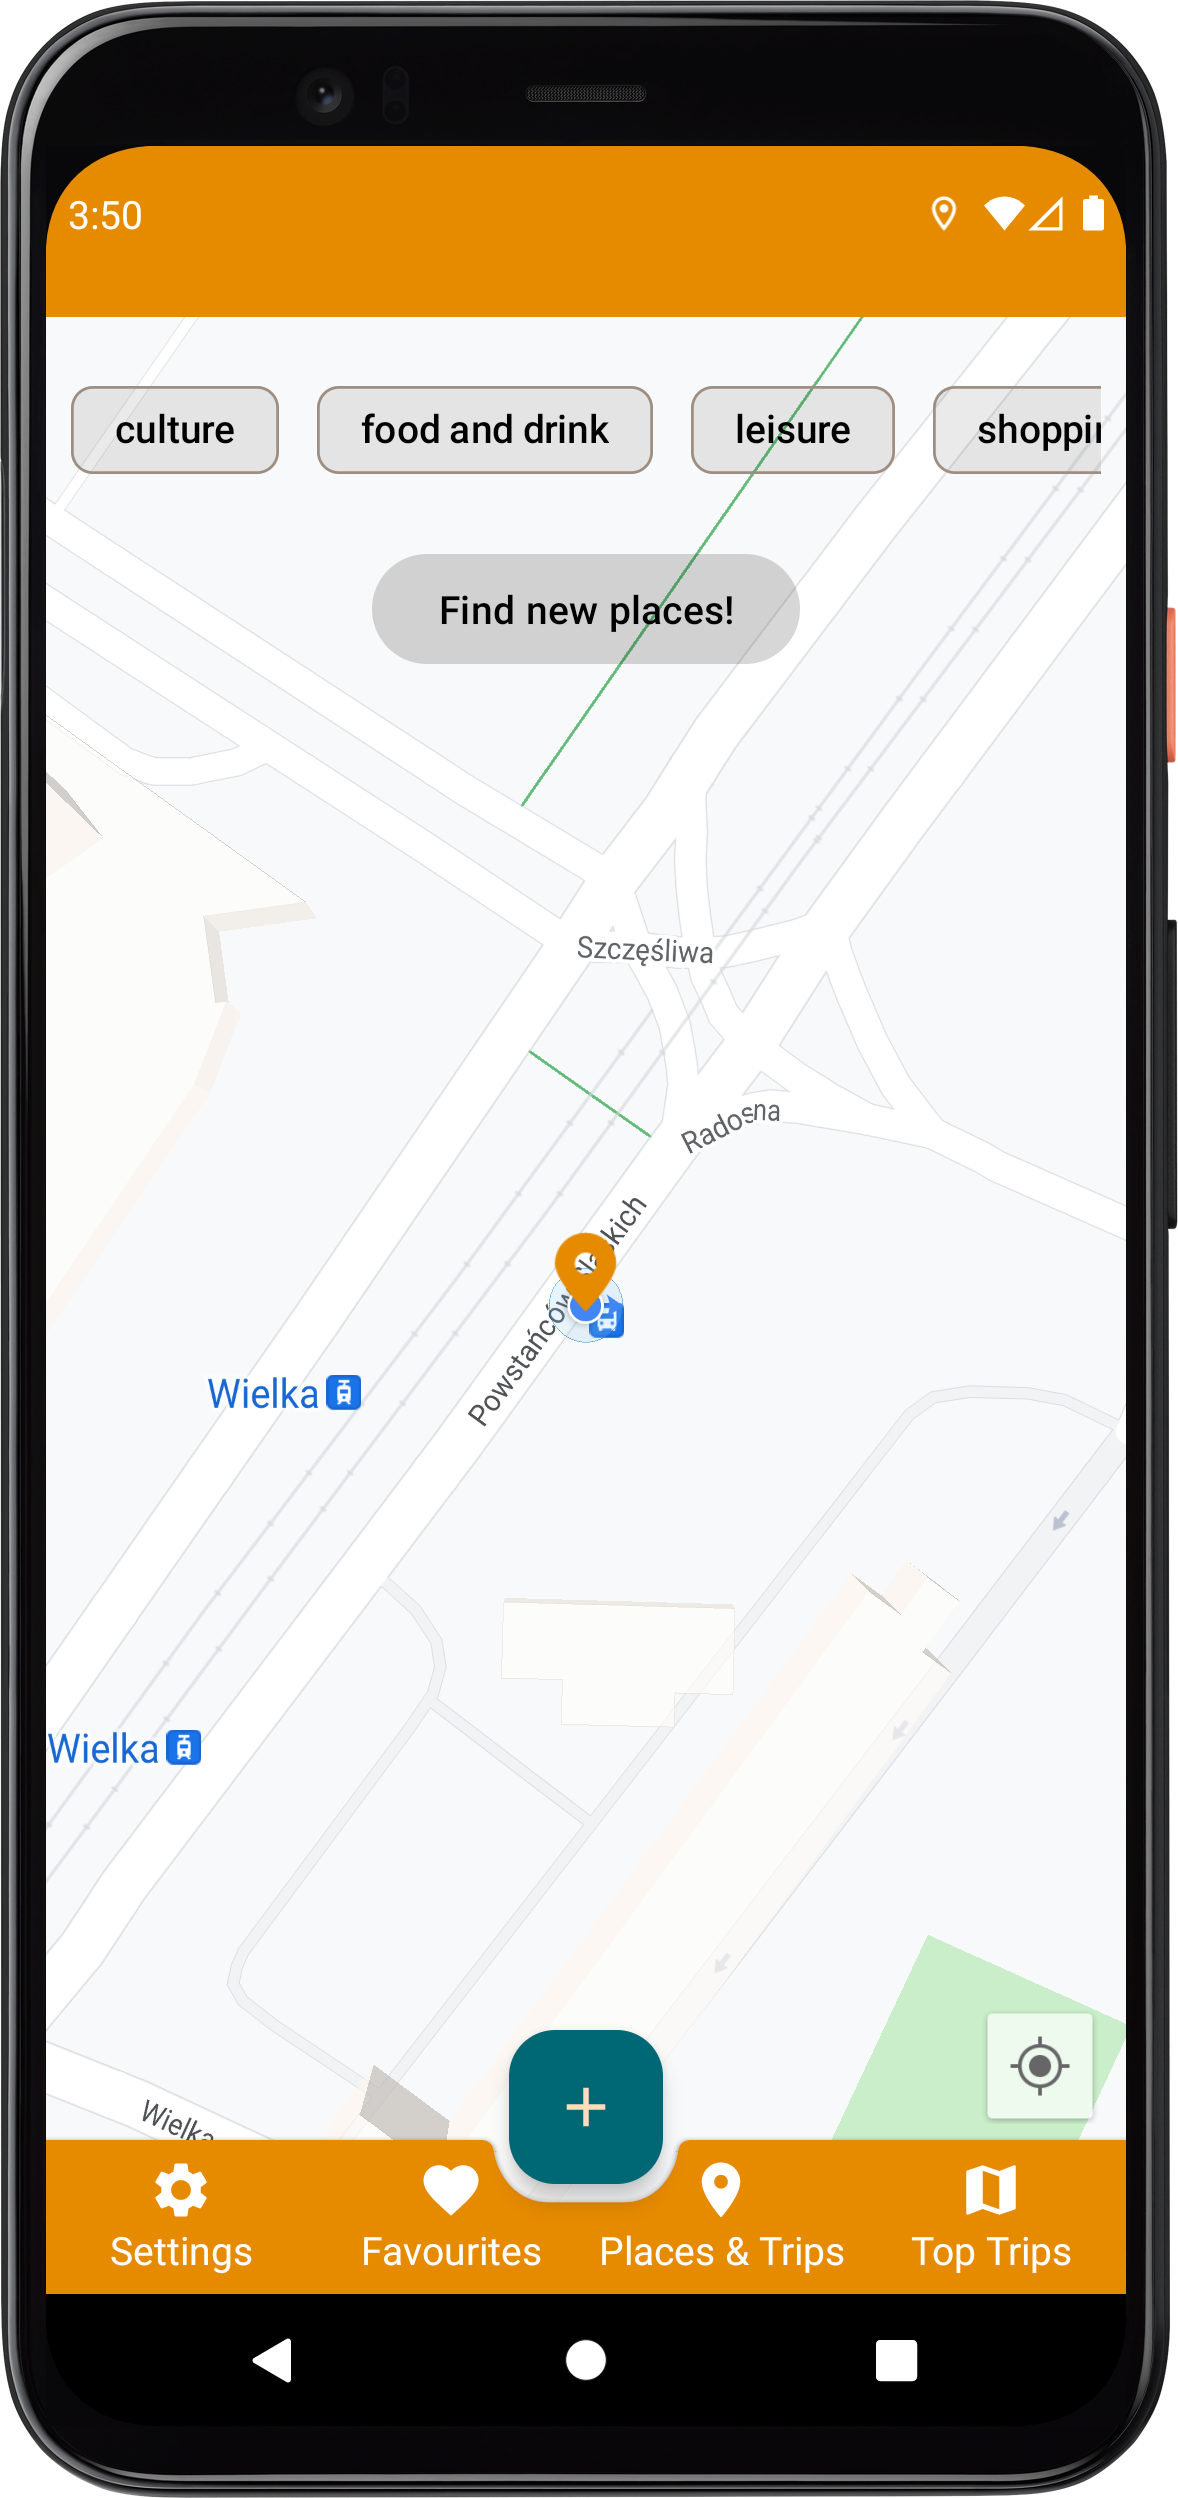
\includegraphics[width=\textwidth]{src/app/map_fragment.png}
                \caption{Pozycja użytkownika widoczna na mapie.\label{map_fragment}}
            \end{subfigure}
            \hfill
            \begin{subfigure}[b]{0.3\textwidth}
                \centering
                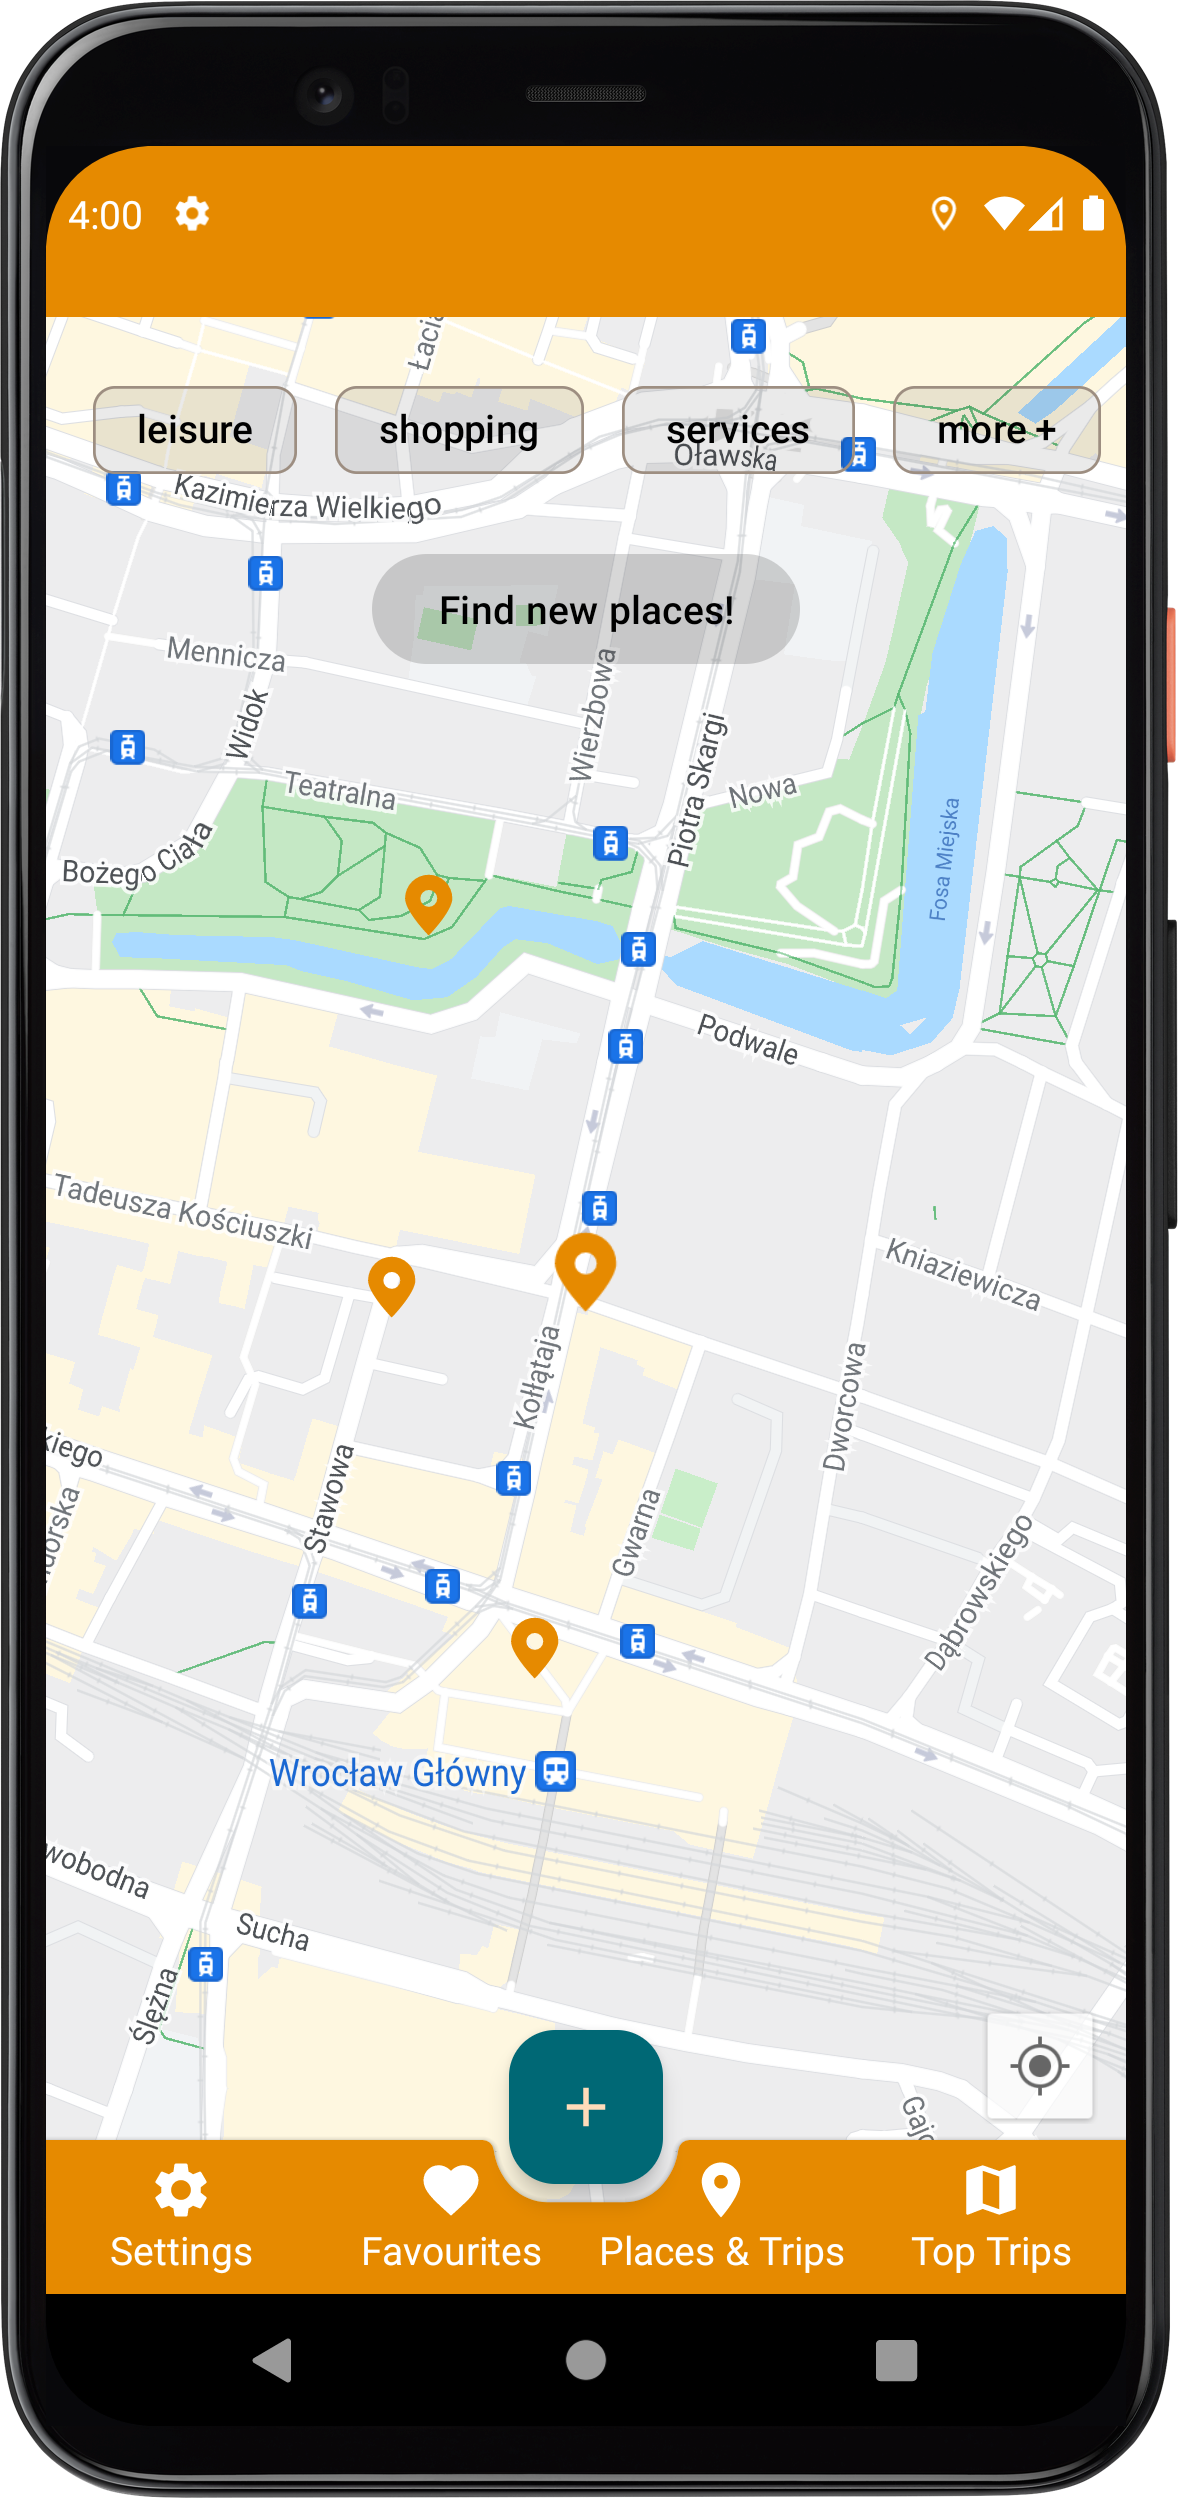
\includegraphics[width=\textwidth]{src/app/find_new_places.png}
                \caption{Wyszukane miejsca oznaczone na mapie.\label{find_places}}
            \end{subfigure}
            \caption{Ekran mapy\label{map}}
            \qquad
        \end{figure} 
        \vspace{1cm}
        
        Ostatni z chipów, opisany „more +” wysuwa dolny arkusz (ang.\@ bottom sheet) zawierający listę etykiet. Za pomocą tego ekranu użytkownik może wybrać do dziesięciu pożądanych przez siebie 
        etykiet. Po wciśnięciu znajdującego się w prawym dolnym rogu ekranu, przycisku szukaj oznaczonego strzałką, na ekranie mapy wyświetlone zostaną miejsca w sposób analogiczny dla przycisku
        „Find new places!”, lecz pobrane zostaną tylko takie, które opisane są wybranymi przez użytkownika etykietami. Na rys.~\ref{tags_empty} zobaczyć można arkusz znaczników. Na rys.~\ref{tags_full}
        widać przykład tego samego ekranu z zaznaczonymi przez użytkownika etykietami. Arkusz etykiet składa się, ze wspomnianych w rozdziale~\ref{interface}, chipów wyboru, które przejrzyście
        obrazują wybór etykiet.

        \vspace{1cm}
        \begin{figure}[H]%
            \centering
            \begin{subfigure}[b]{0.3\textwidth}
                \centering
                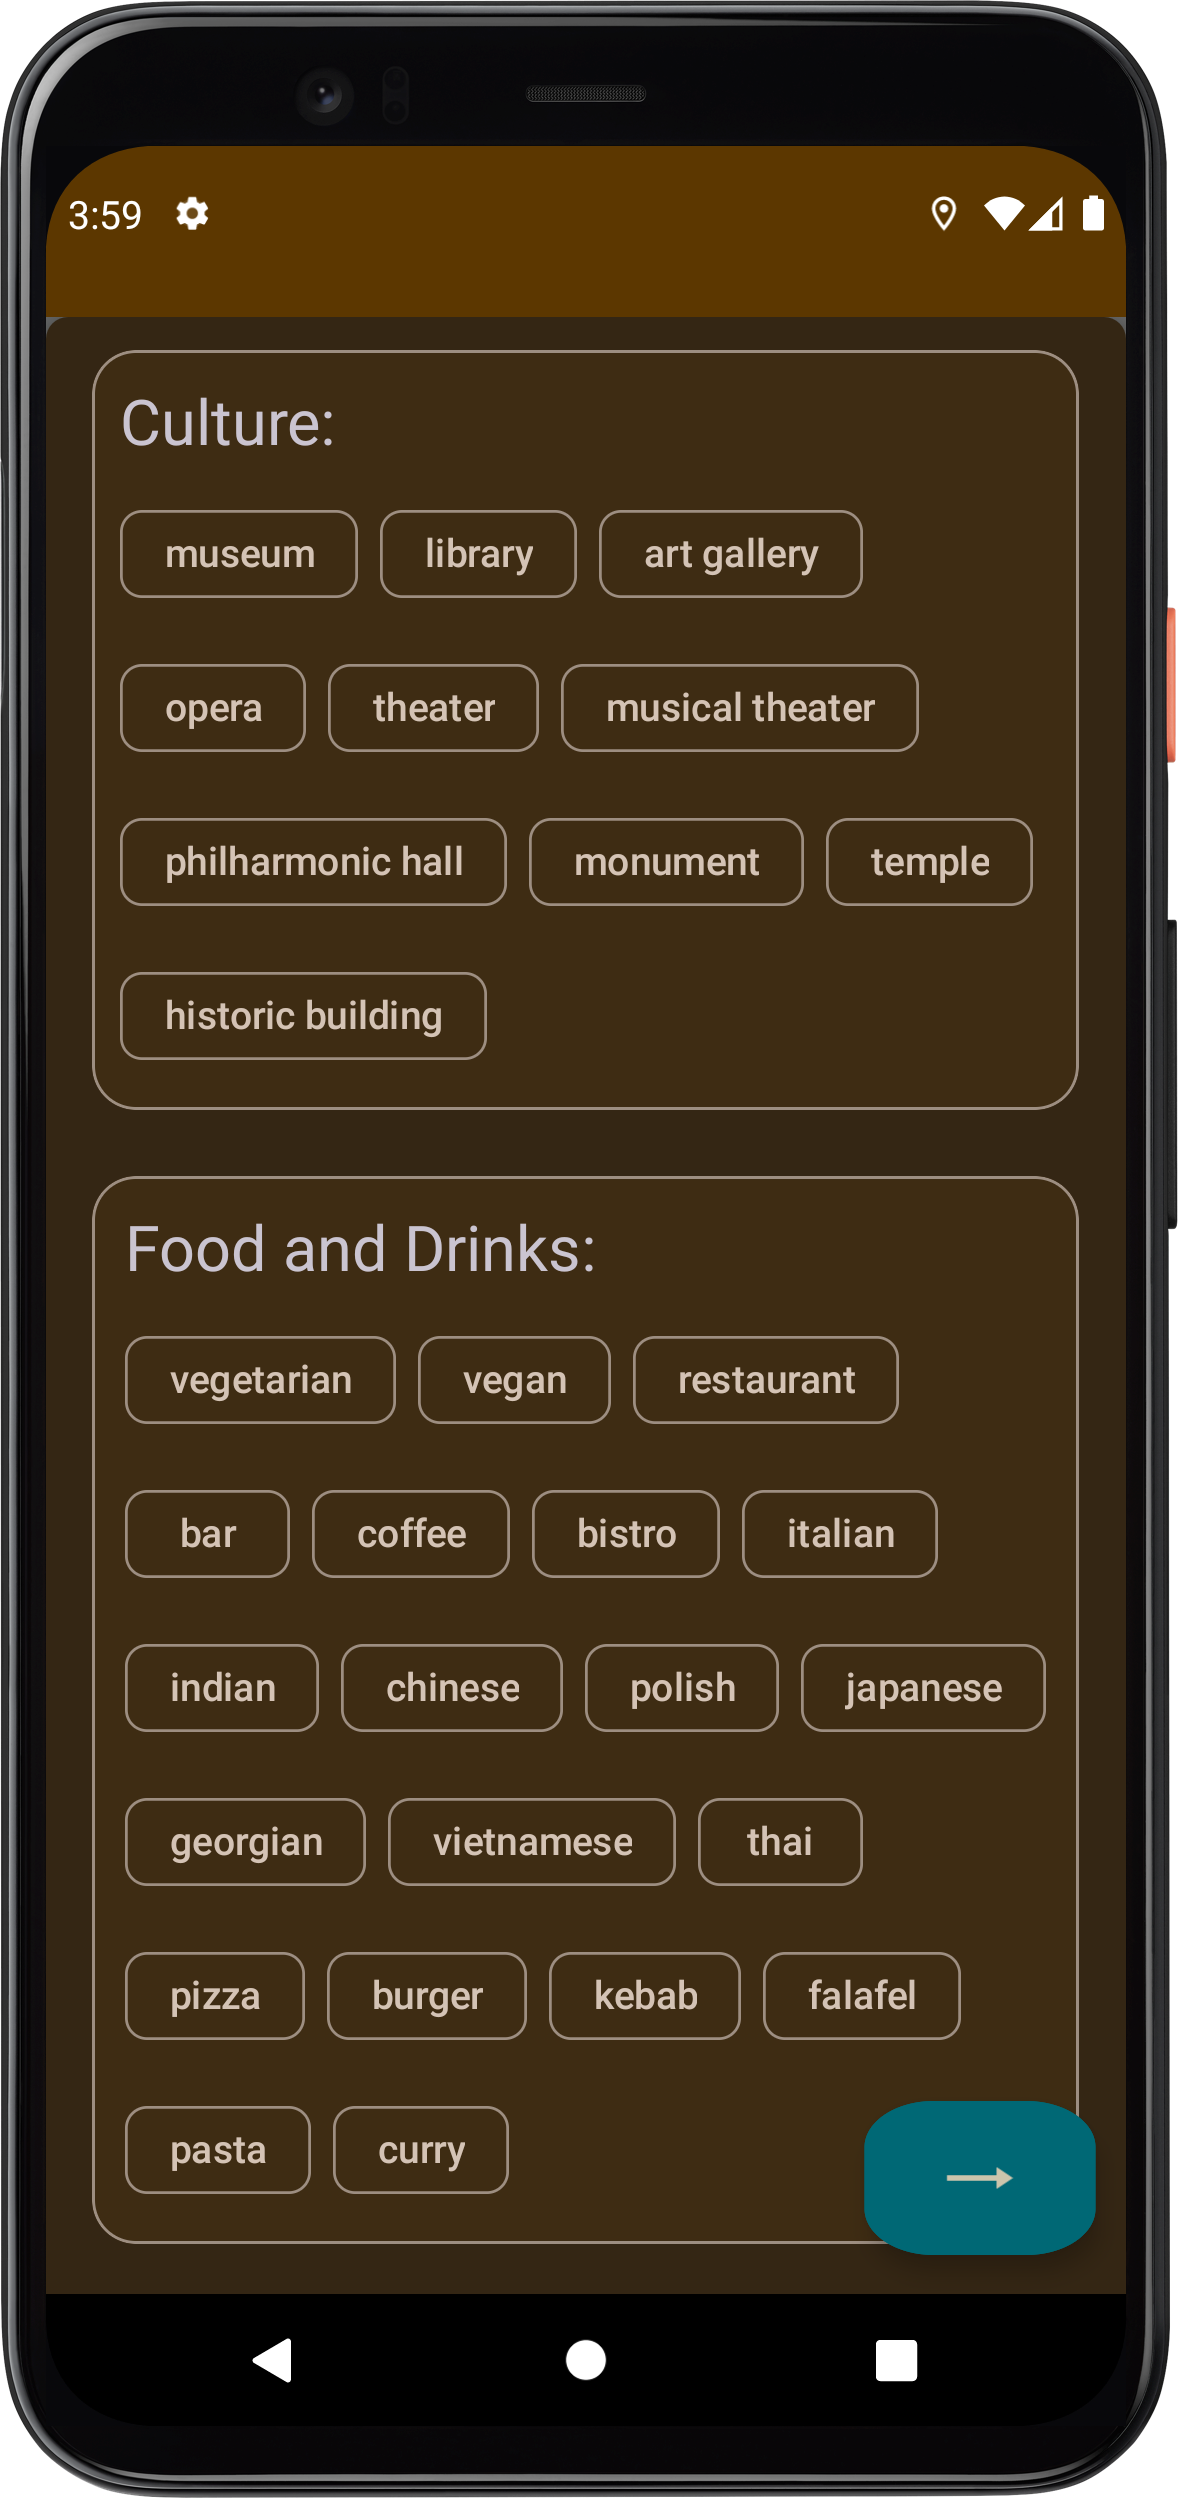
\includegraphics[width=\textwidth]{src/app/tags_unselected.png}
                \caption{Czysty arkusz etykiet.\label{tags_empty}}
            \end{subfigure}
            \hfill
            \begin{subfigure}[b]{0.3\textwidth}
                \centering
                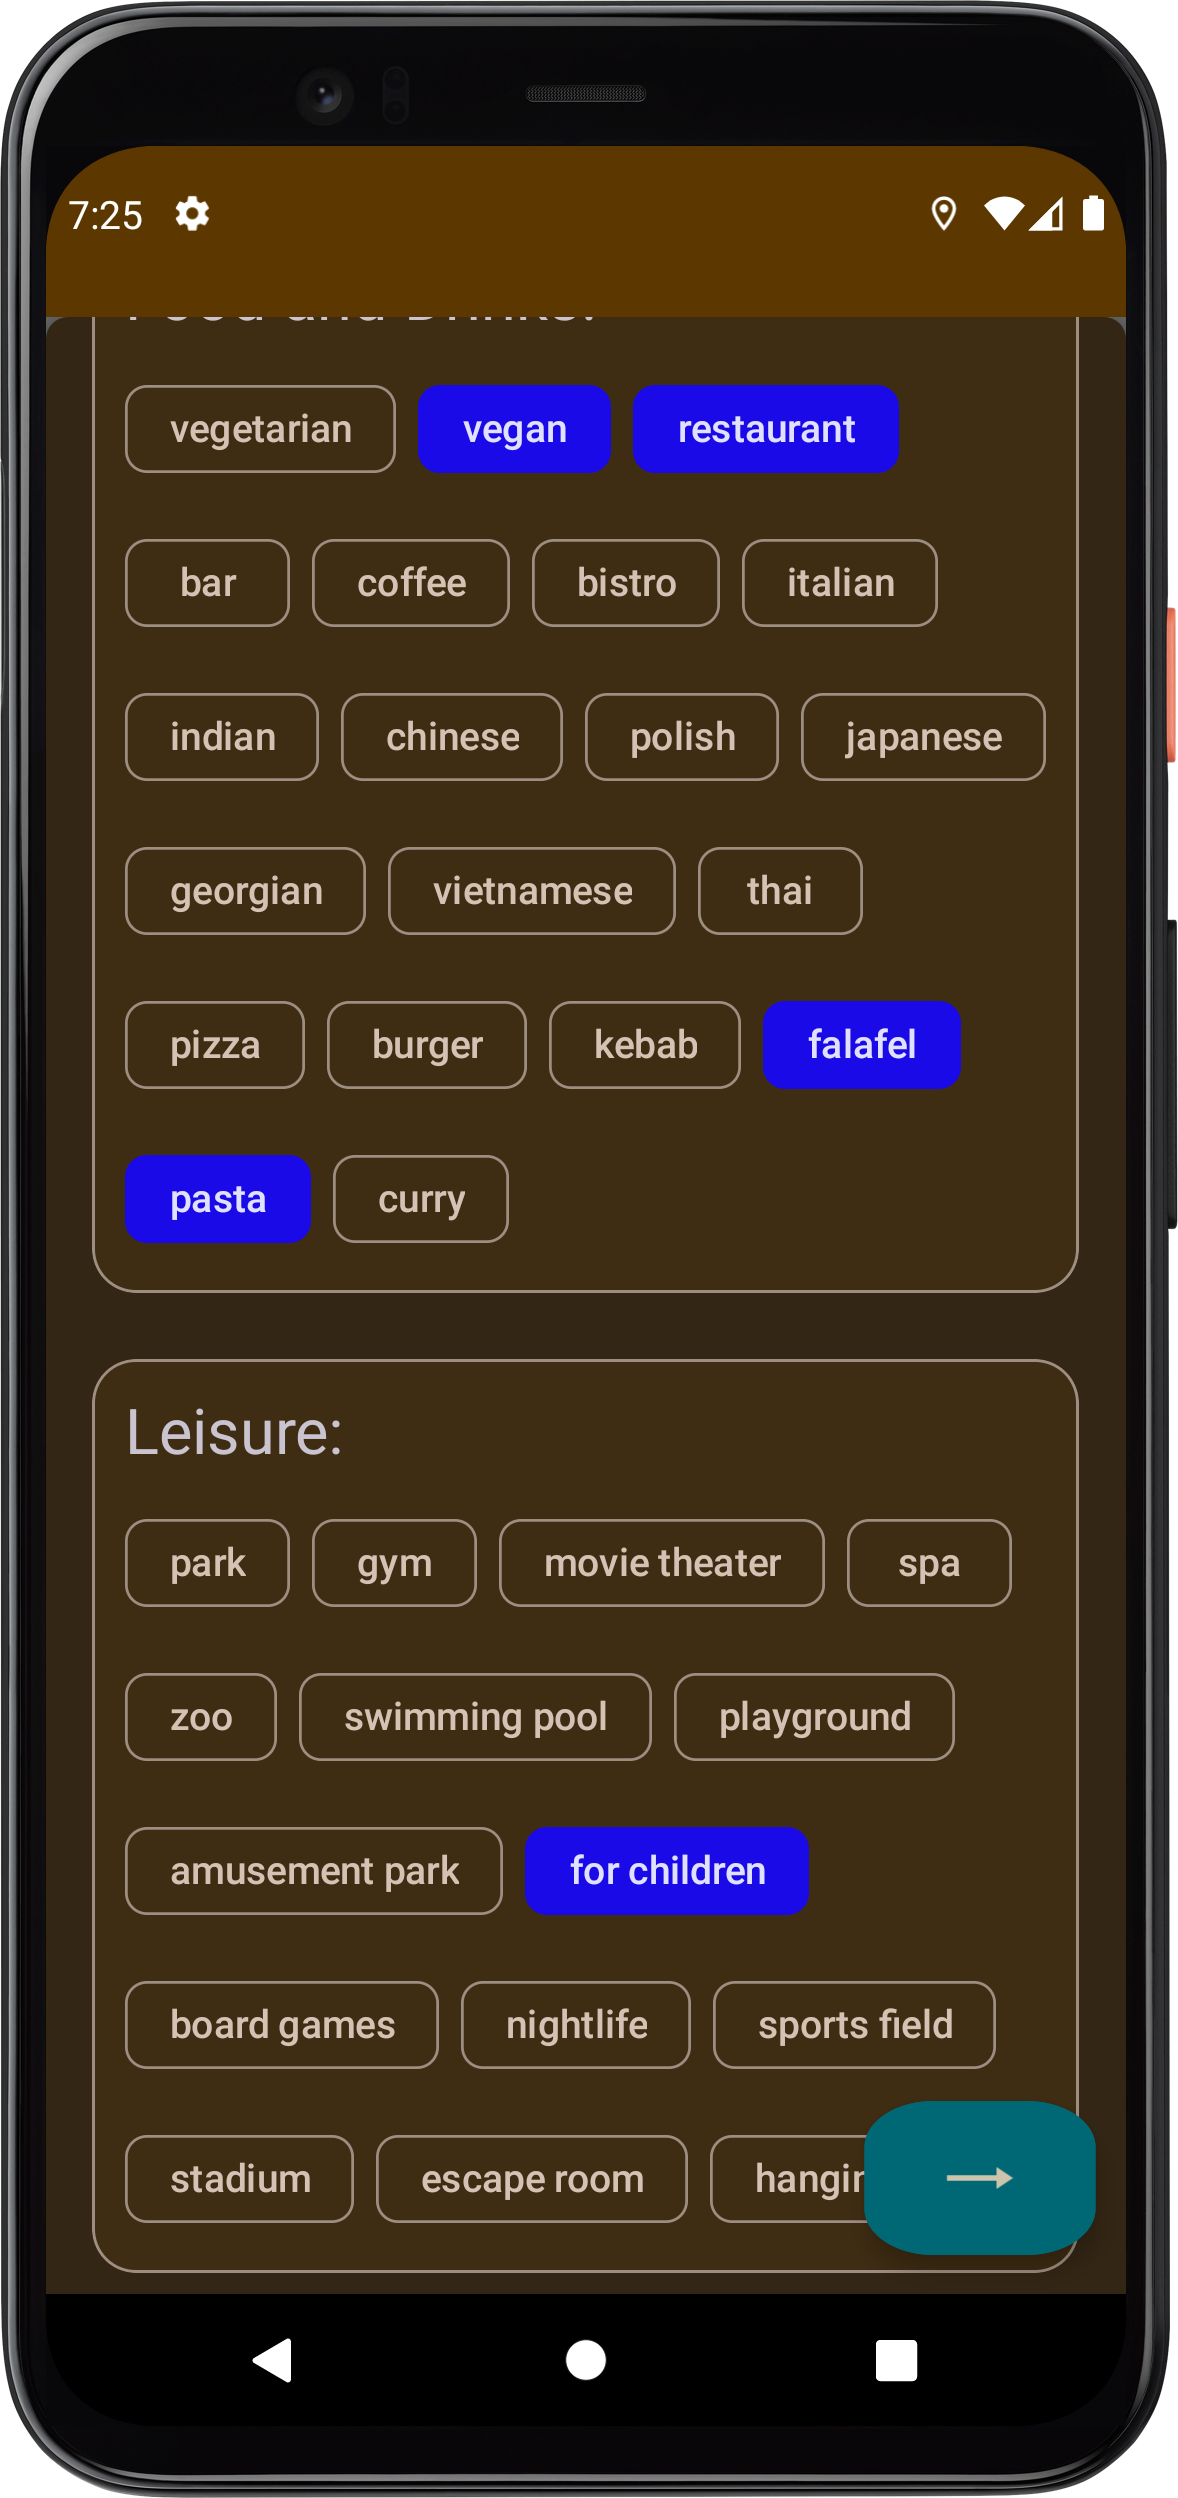
\includegraphics[width=\textwidth]{src/app/tags_selected.png}
                \caption{Arkusz etykiet z wyborami użytkownika.\label{tags_full}}
            \end{subfigure}
            \caption{Dolny arkusz etykiet.\label{tags}}
            \qquad
        \end{figure} 
        \vspace{1cm}

        Na środku ekranu znajduje się duża pomarańczowa pinezka, której igła zaznacza środek ekranu. Służy ona za kursor w trakcie dodawania miejsca. Na środkowym dole ekranu znajduje się oznaczony 
        plusem przycisk dodania miejsca. Rozpoczyna on proces dodawania miejsca, znajdującego się w miejscu wskazanym przez kursor. Po wciśnięciu na ekranie pojawia się okno dialogowe z polami, które uzupełnić
        musi użytkownik, aby dodać miejsce do bazy danych. Użytkownik musi sprecyzować jego nazwę, opis oraz wybrać co najmniej jedną z pięciu możliwych kategorii. Dialog tworzenia miejsca widoczny jest na 
        rys.~\ref{place_empty}. Przykład poprawnie wypełnionego ekranu tworzenia miejsca widoczny jest na rys.~\ref{place_filled}

        \vspace{1cm}
        \begin{figure}[H]%
            \centering
            \begin{subfigure}[b]{0.3\textwidth}
                \centering
                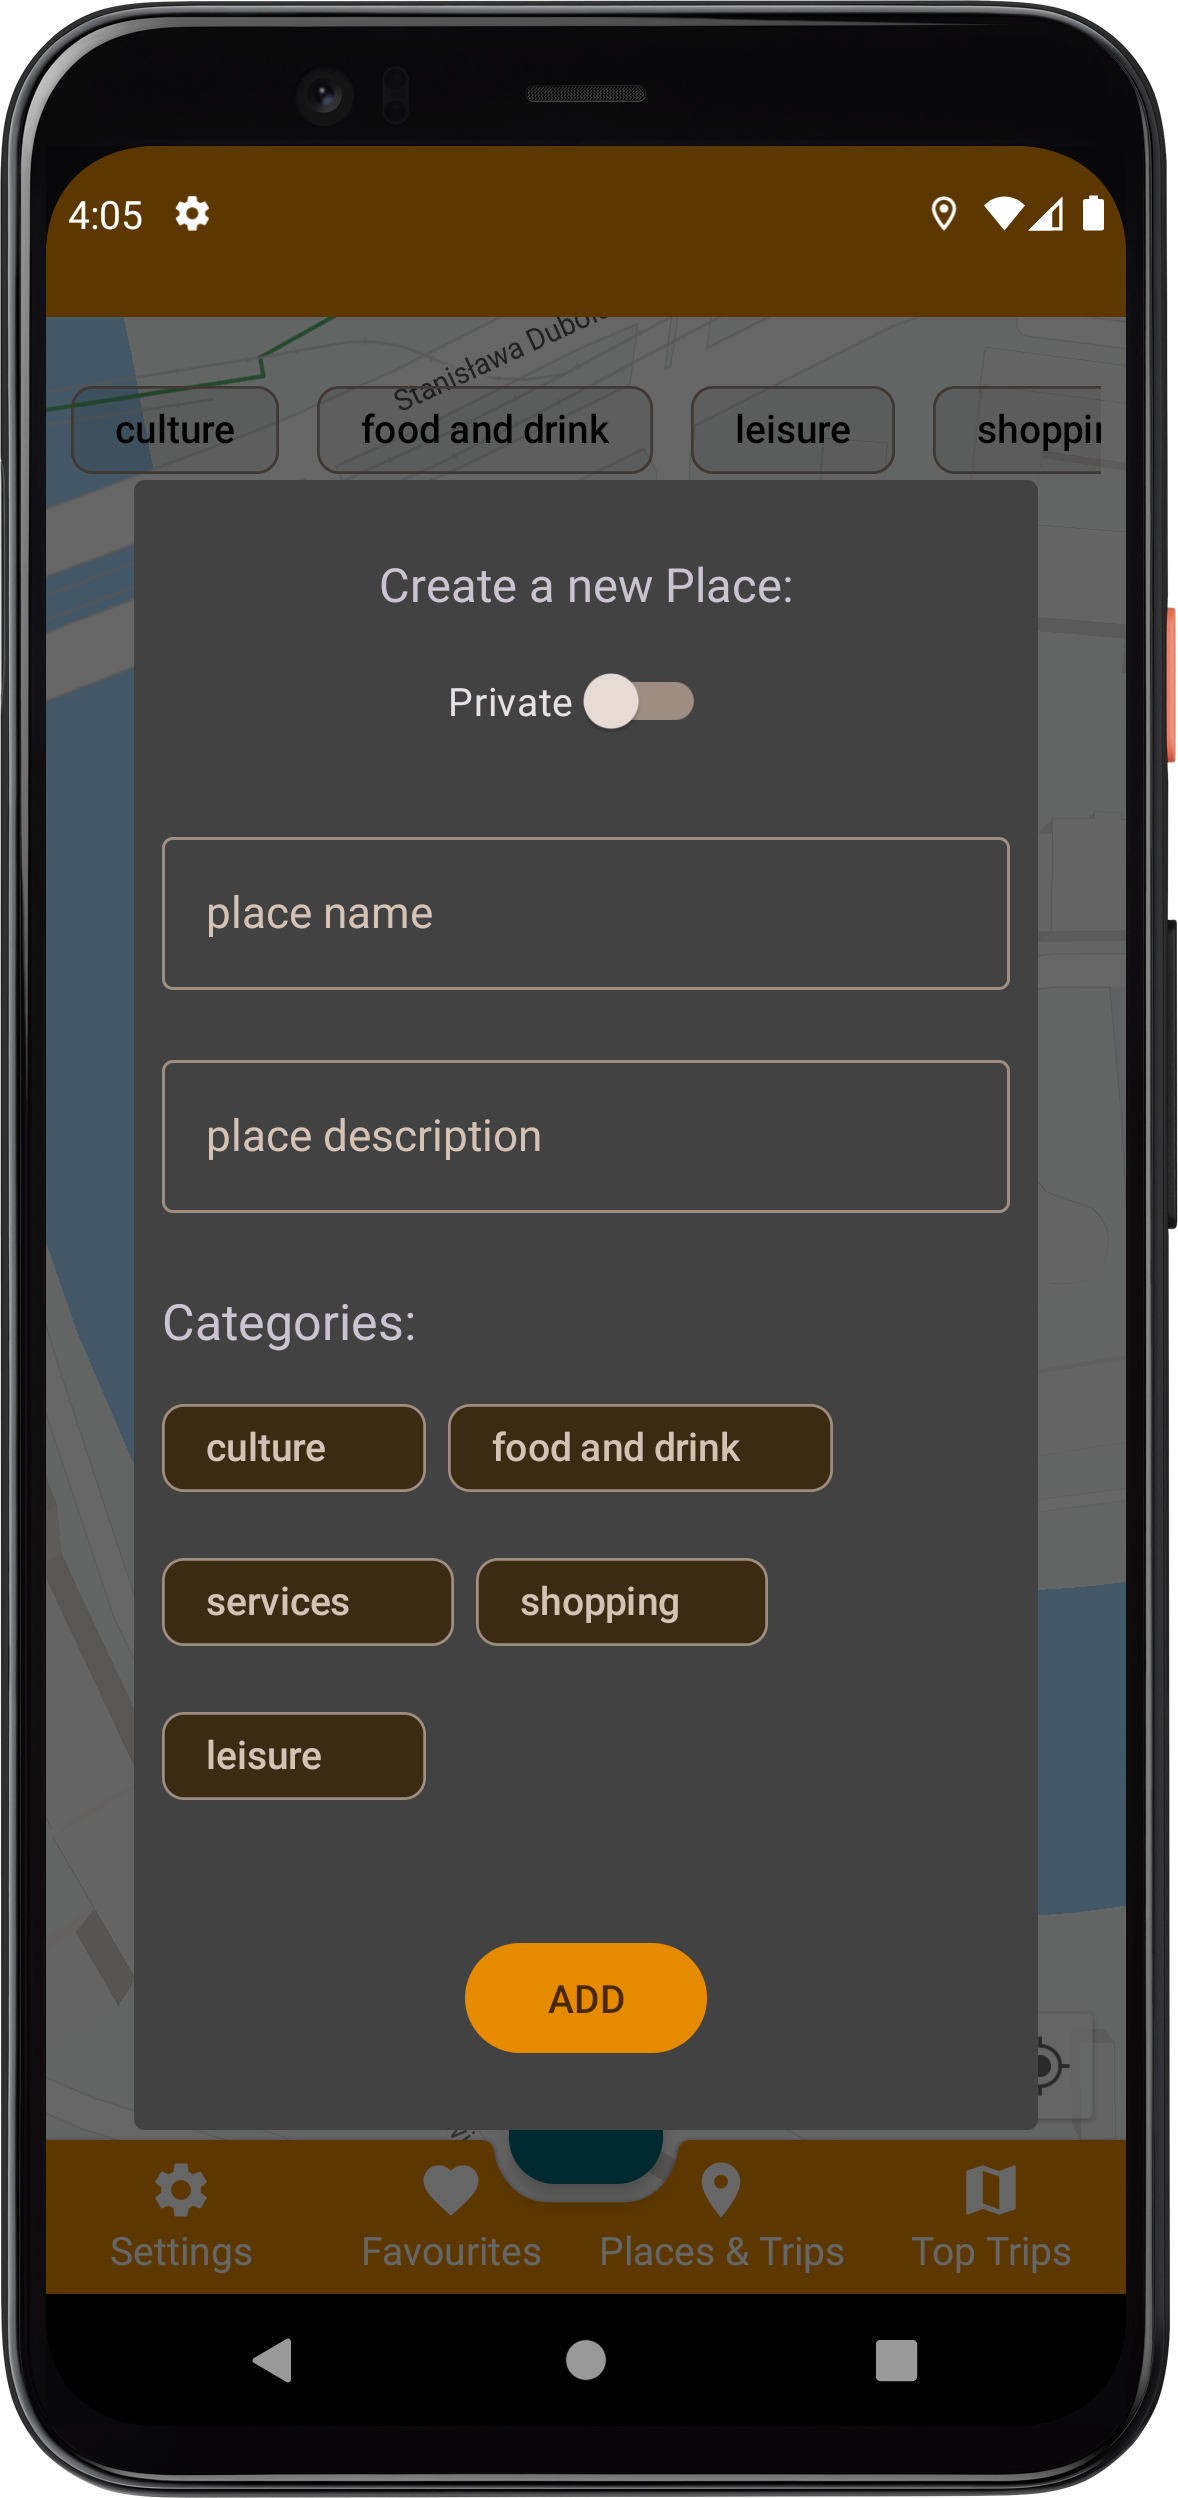
\includegraphics[width=\textwidth]{src/app/add_place1.png}
                \caption{Pusty dialog.\label{place_empty}}
            \end{subfigure}
            \hfill
            \begin{subfigure}[b]{0.3\textwidth}
                \centering
                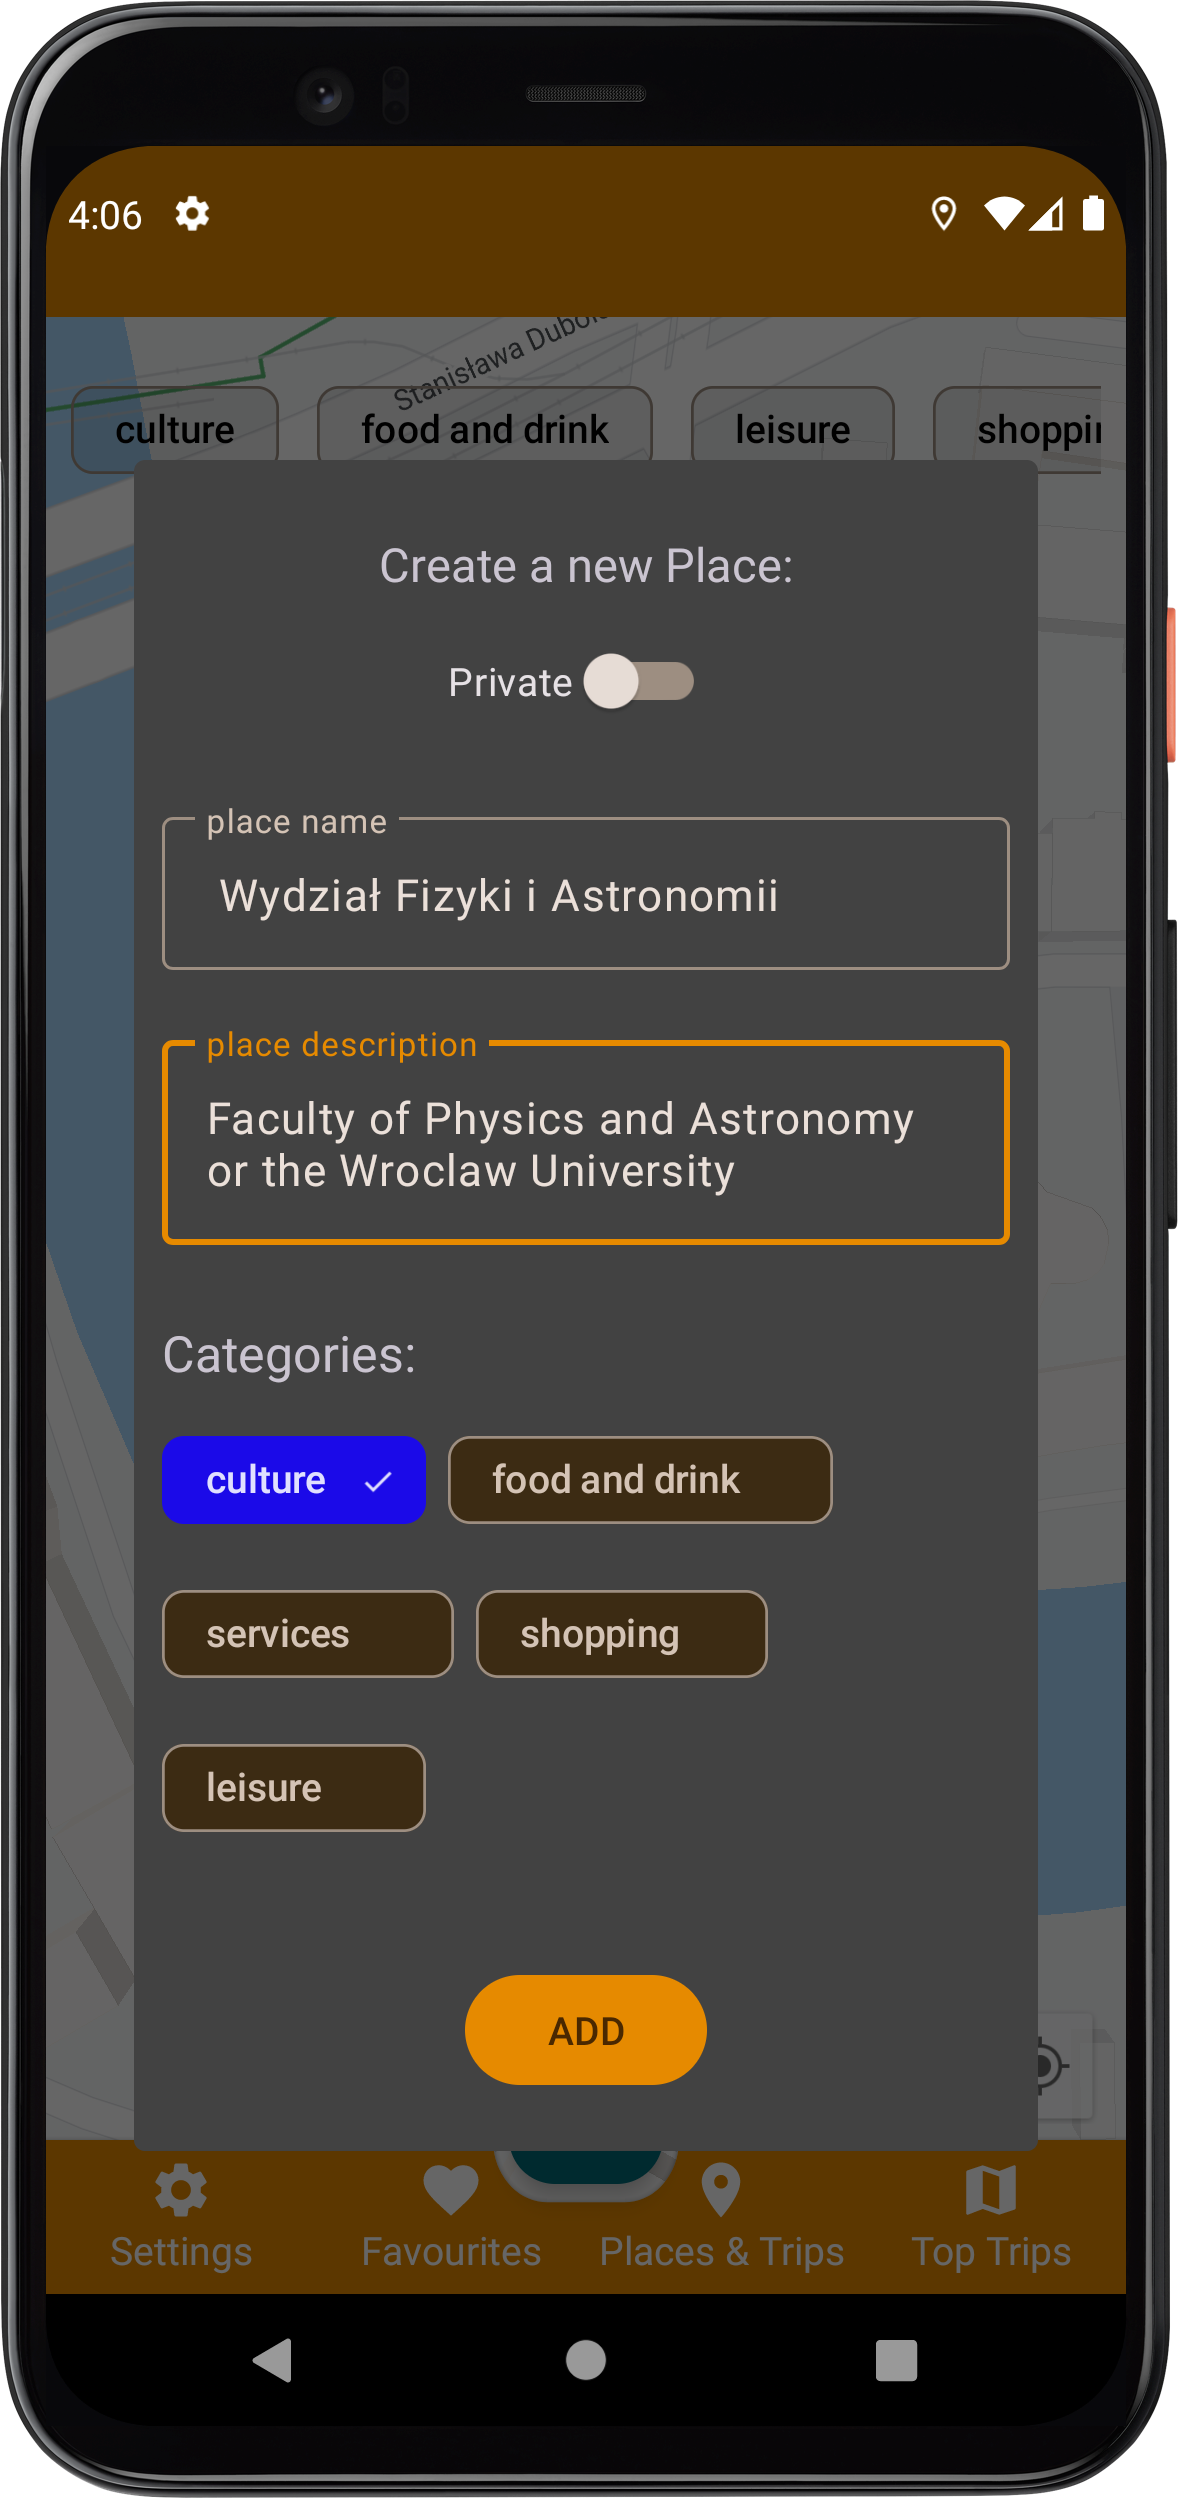
\includegraphics[width=\textwidth]{src/app/add_place2.png}
                \caption{Wypełniony dialog.\label{place_filled}}
            \end{subfigure}
            \caption{Dialog tworzenia miejsca.\label{add_place}}
            \qquad
        \end{figure} 
        \vspace{1cm}

        Jak zauważyć można na rys.~\ref{find_places}, wyszukane miejsca pojawiają się na mapie w formie pinezek. Kliknięcie pinezki otwiera dolny arkusz przedstawiający detale miejsca. 
        Na górze ekranu widoczne są nazwa miejsca, jego autor i wybrane przez niego kategorie. W prawym górnym rogu znajduje się licznik polubień i przycisk w kształcie serca, za pomocą którego użytkownik
        może dodać miejsce do swoich ulubionych. Poniżej kategorii widoczna jest lista etykiet z licznikami dodań. Pod nimi znajduje się przycisk dodania etykiet. Otwiera on arkusz widoczny wcześniej podczas
        wyszukiwania na rys.~\ref{tags}. Tym razem na miejscu przycisku wyszukania widoczny jest przycisk dodania oznaczony plusem sugerujący zmianę akcji na dodawanie etykiet. Na prawo od przycisku dodawania
        etykiet znajduje się oznaczony obrazkiem znaku drogowego przycisk rysowania drogi. Zamyka on arkusz miejsca i rysuję na mapie trasę rozpoczynającą się w aktualnej pozycji użytkownika, a kończącą w
        wybranym miejscu. Przesuwanie palcem w prawo lub w lewo zaskutkuje zmianą aktualnie wyświetlanego miejsca na inne znajdujące się w jego okolicy. Arkusz detali miejsca widoczny jest na 
        rys.~\ref{place}.

        \vspace{1cm}
        \begin{figure}[H]
            \centering
            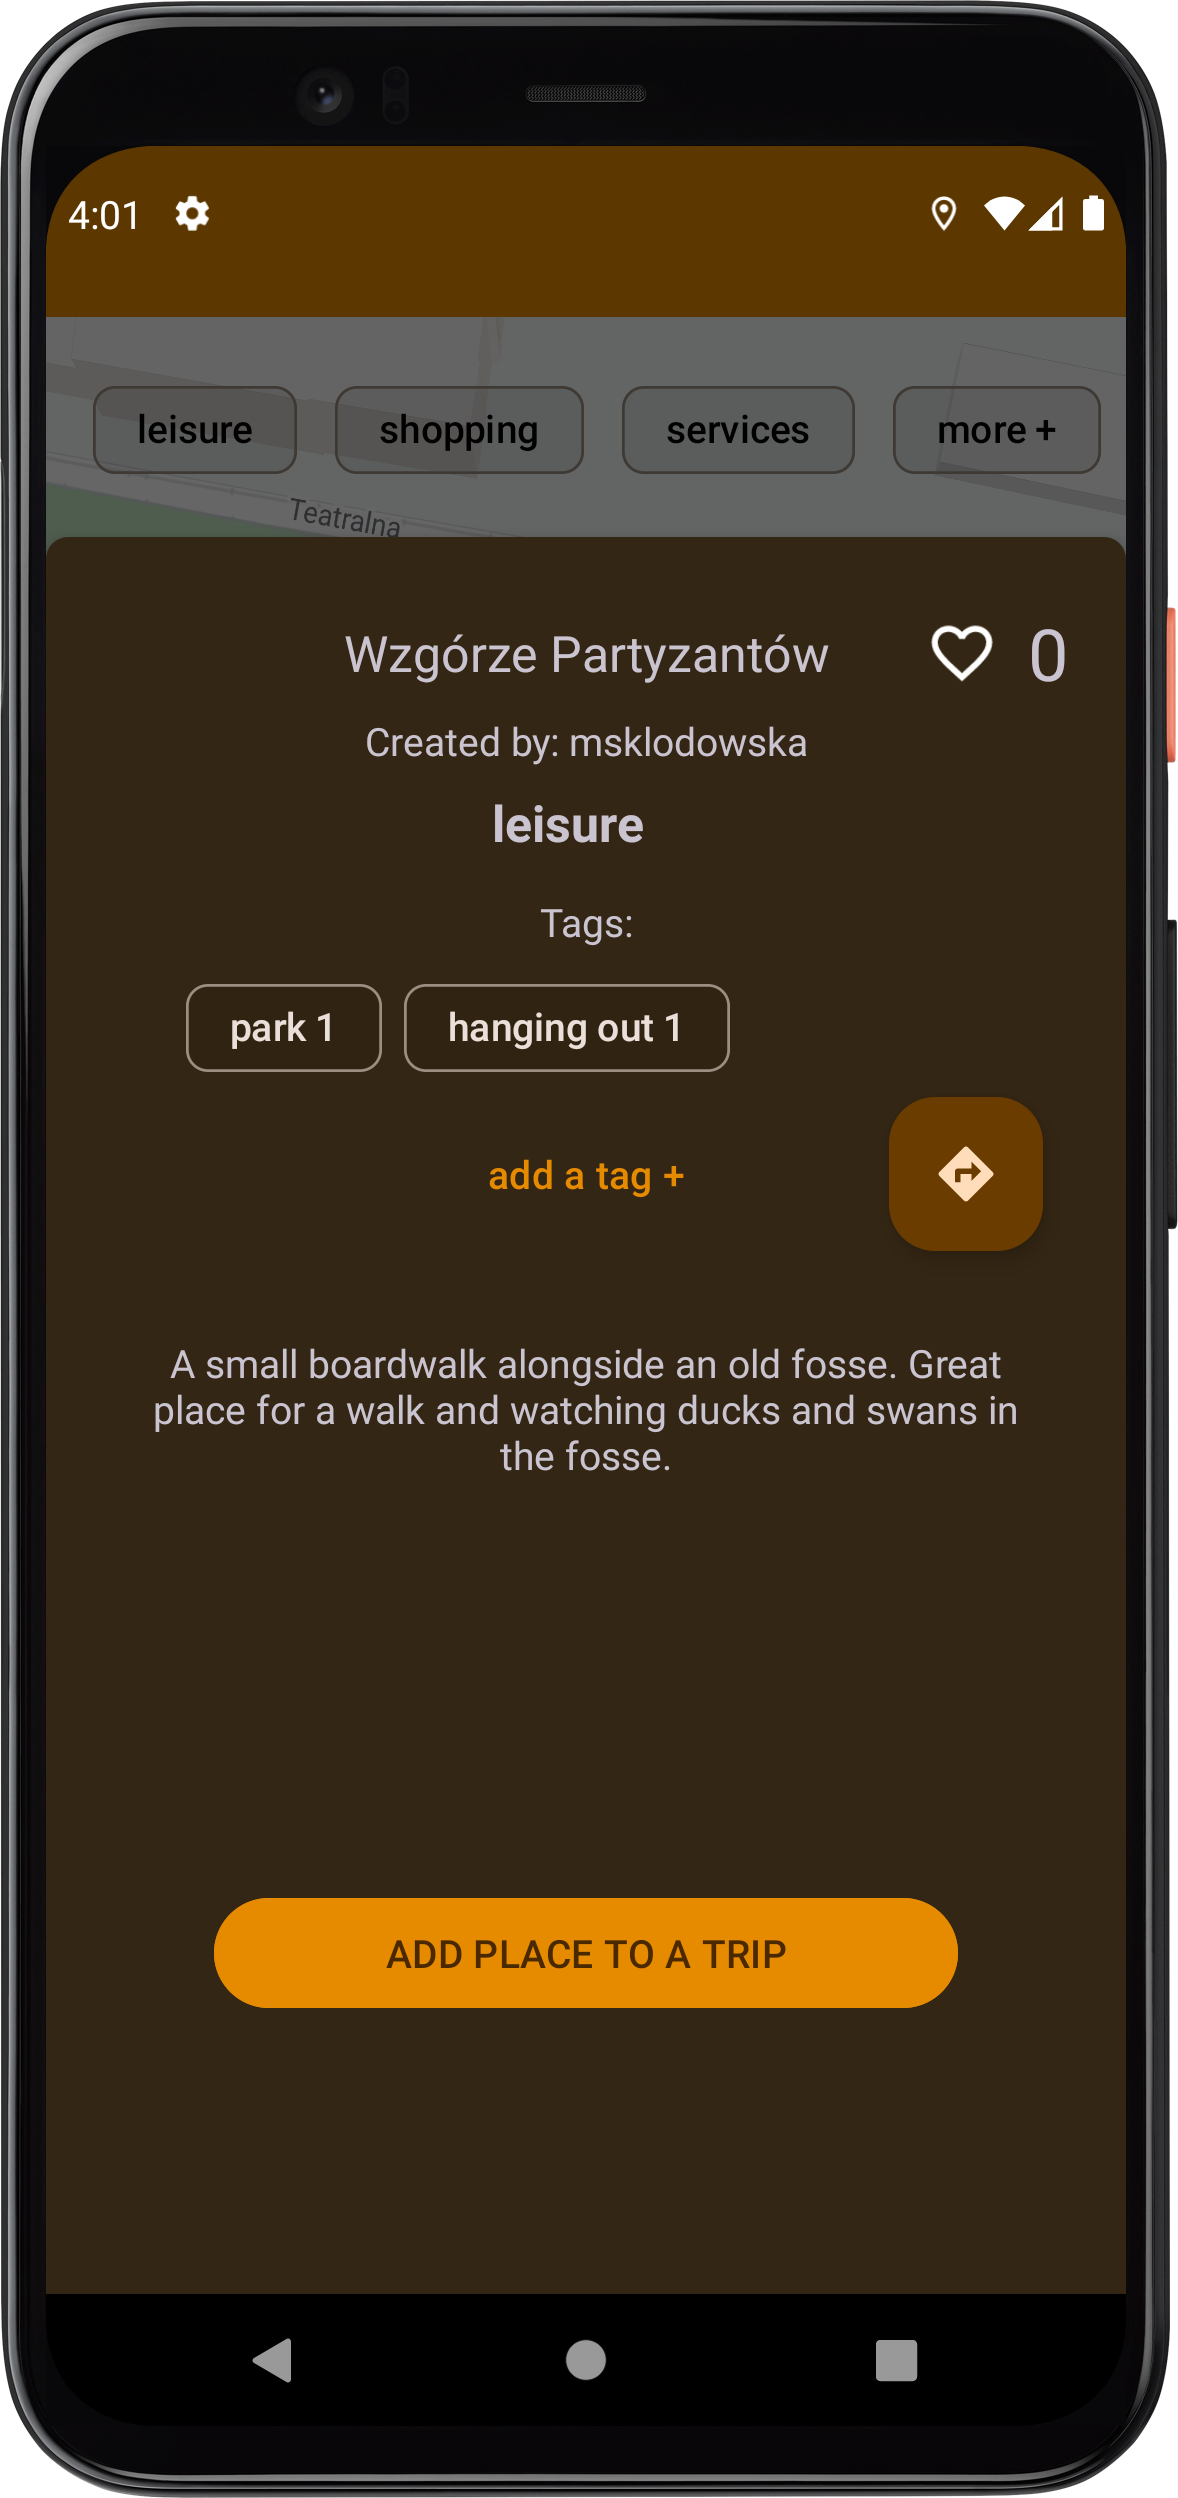
\includegraphics[scale=0.10]{src/app/place_viewer.png}
            \caption{Widok szczegółów miejsca.\label{place}}
            \qquad
        \end{figure} 
        \vspace{1cm}

        Na samym dole arkusza miejsca użytkownik ma możliwość dodania go do wycieczki. Wciśnięcie przycisku wywoła ekran dialogowy, widoczny na rysunku~\ref{trip_dialog} 
        dający użytkownikowi wybór pomiędzy dodaniem miejsca do istniejącej wycieczki lub utworzeniem nowej wycieczki zawierającej wybrane miejsce. Opcja istniejącej wycieczki
        przedstawi użytkownikowi listę wszystkich utworzonych przez niego wycieczek widoczną na rys.~\ref{trip_exist}. Wciskając element listy, użytkownik doda do niej wybrane miejsce 
        i zakończy proces. Druga z opcji otworzy formularz tworzenia nowej wycieczki, w którym użytkownik może ustalić jej prywatność oraz nadać jej nazwę i opis.

        \vspace{1cm}
        \begin{figure}[H]
            \centering
            \begin{subfigure}[b]{0.3\textwidth}
                \centering
                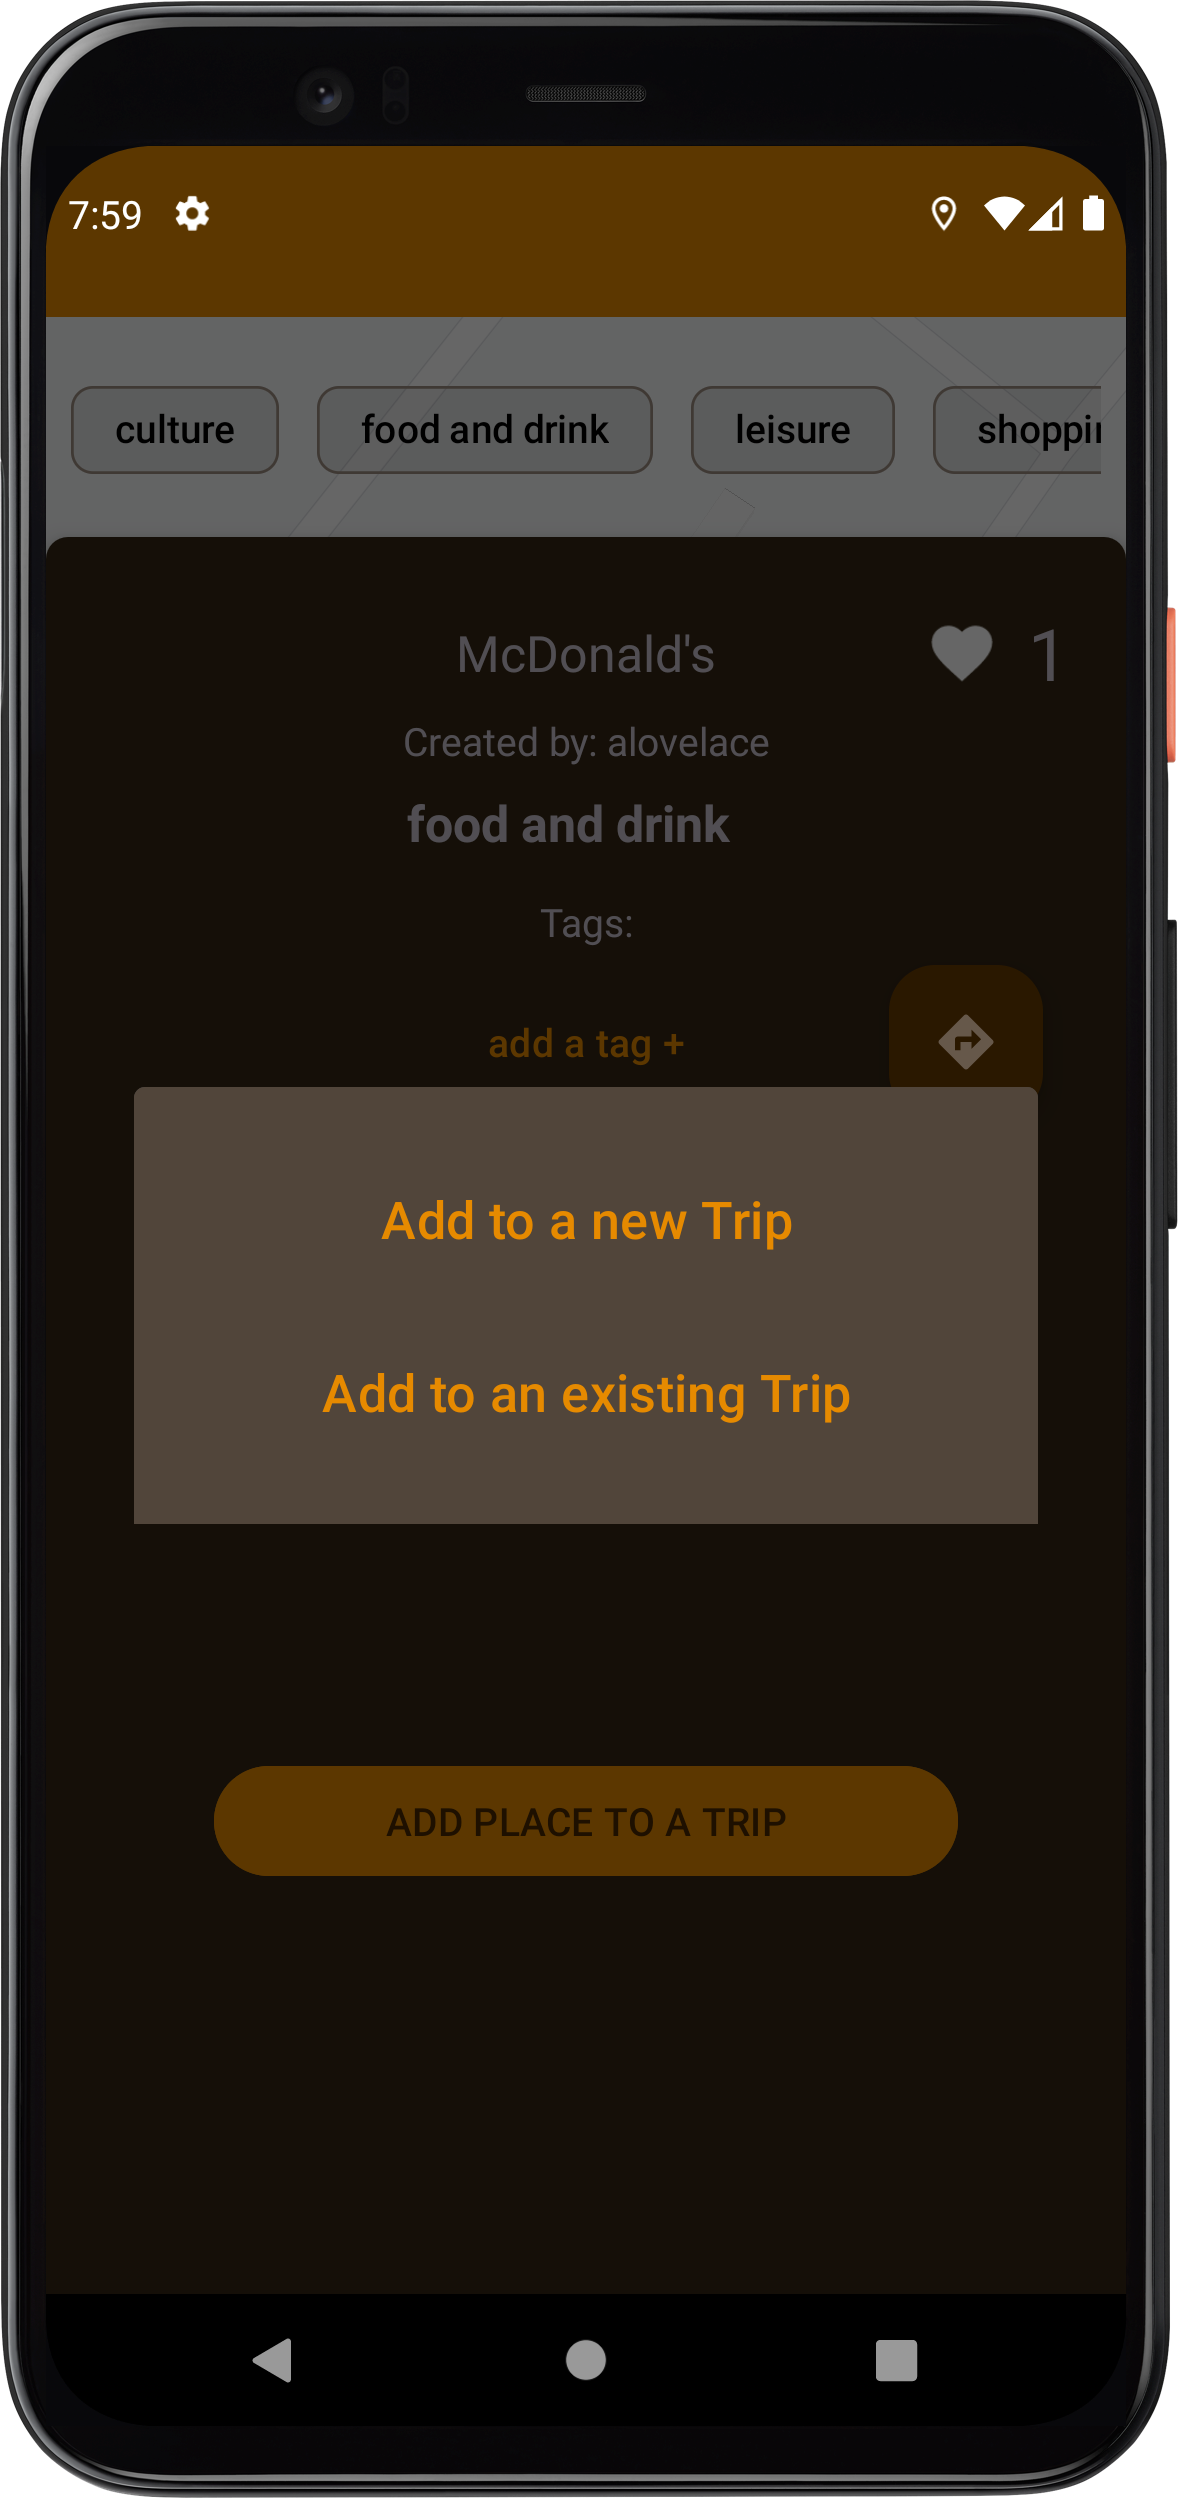
\includegraphics[width=\textwidth]{src/app/trip_dialog.png}
                \caption{Wybór akcji dodawania wycieczki.\label{trip_dialog}}
            \end{subfigure}
            \hfill
            \begin{subfigure}[b]{0.3\textwidth}
                \centering
                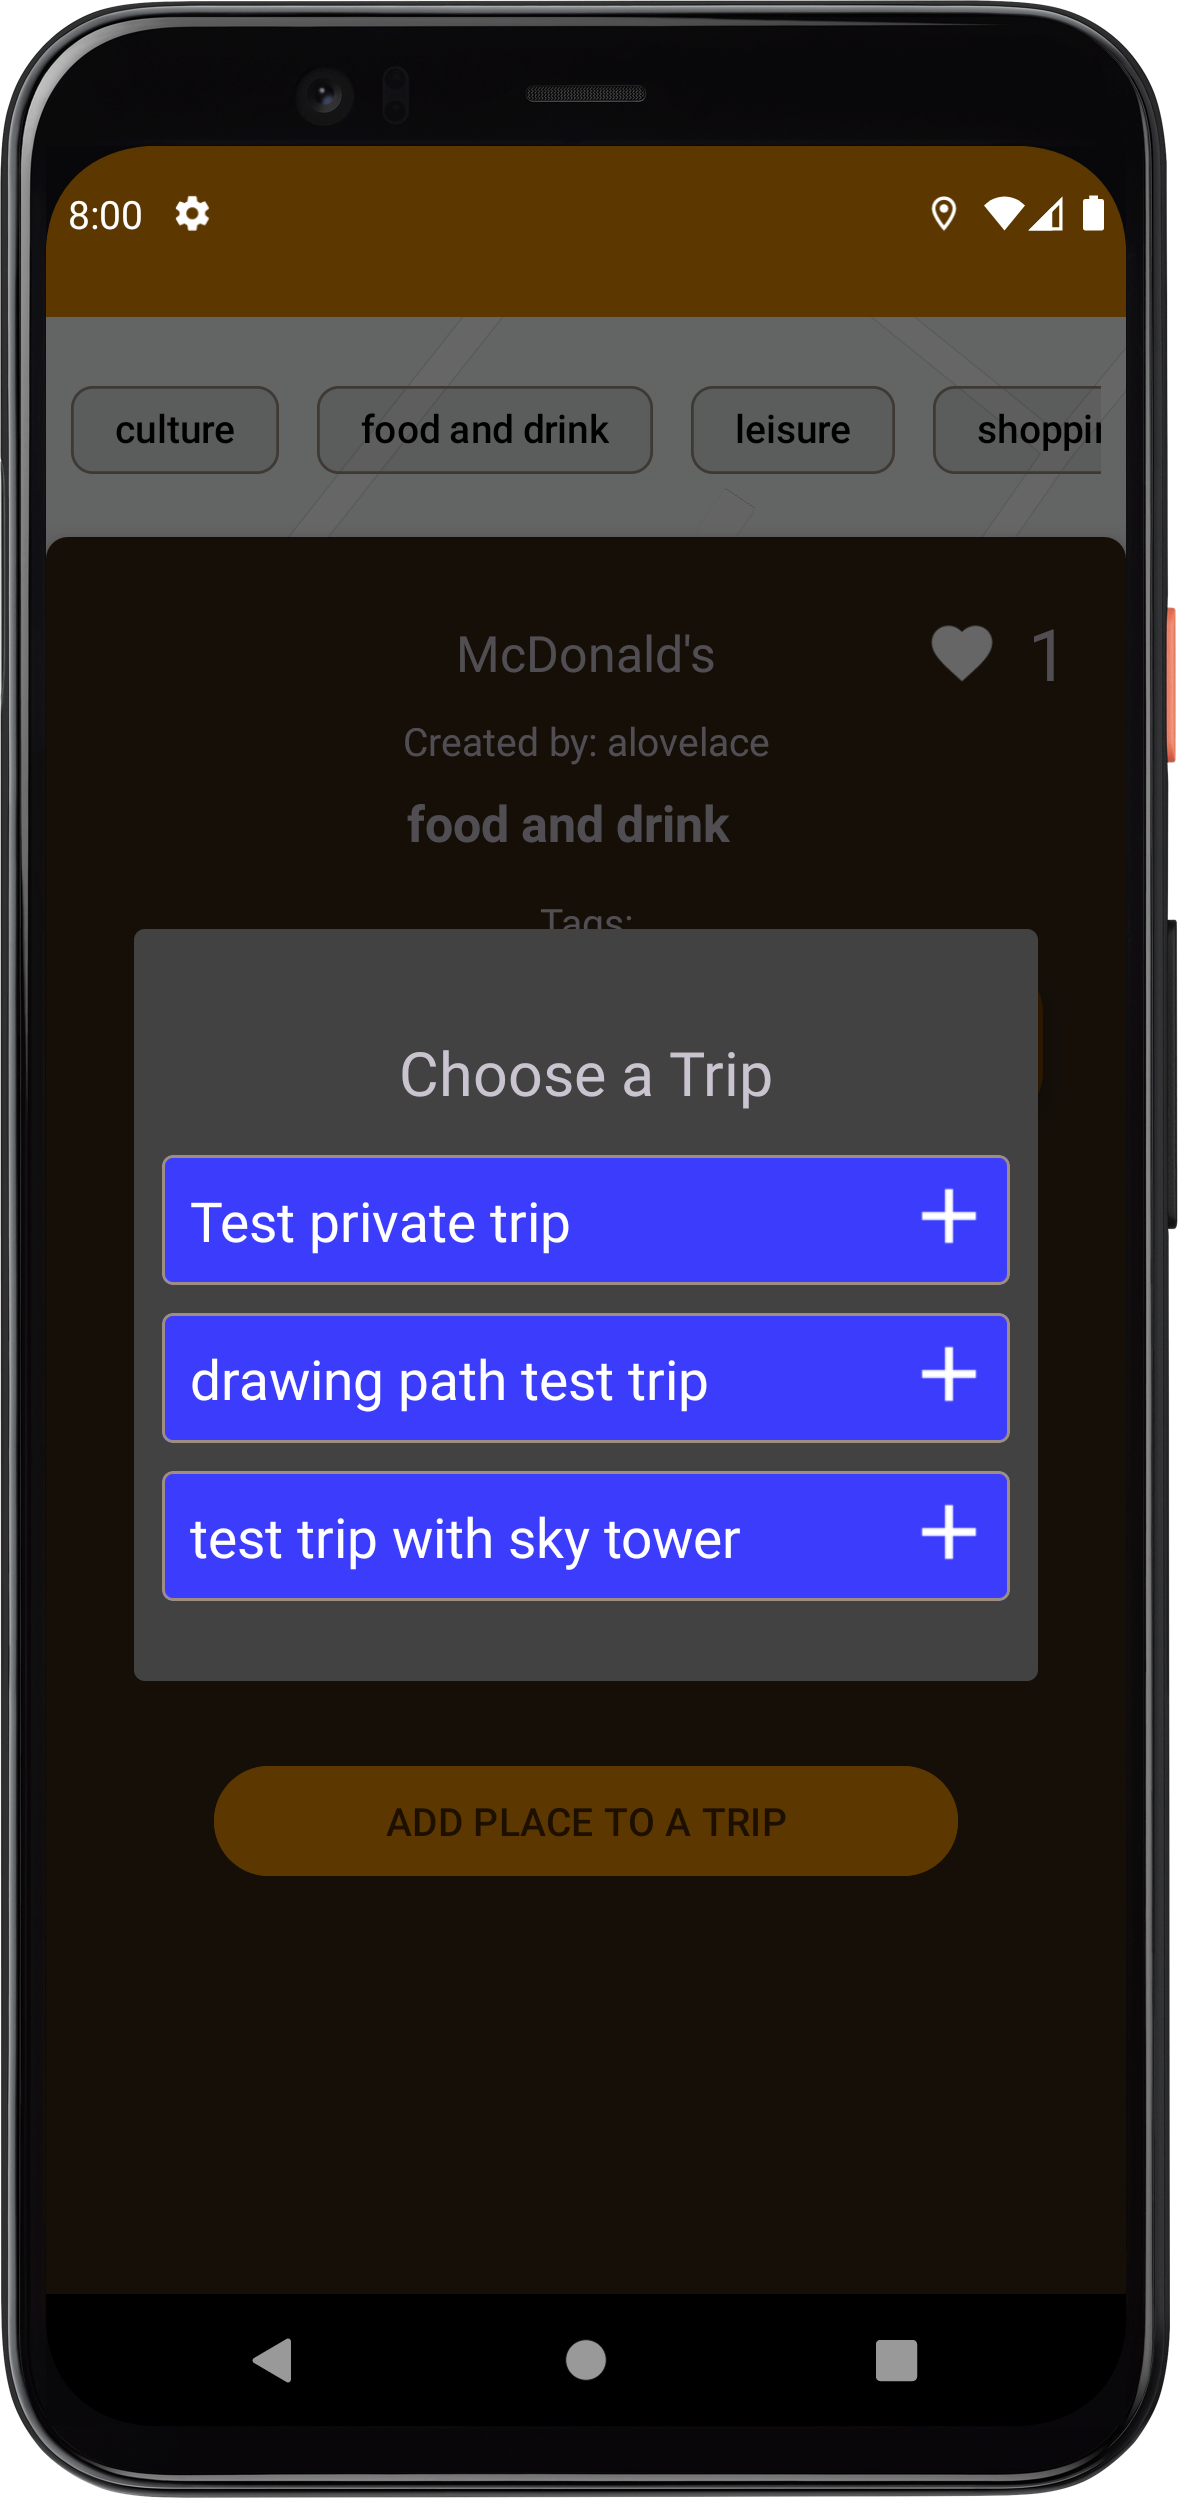
\includegraphics[width=\textwidth]{src/app/existing_trip.png}
                \caption{Lista istniejących wycieczek.\label{trip_exist}}
            \end{subfigure}
            \hfill
            \begin{subfigure}[b]{0.3\textwidth}
                \centering
                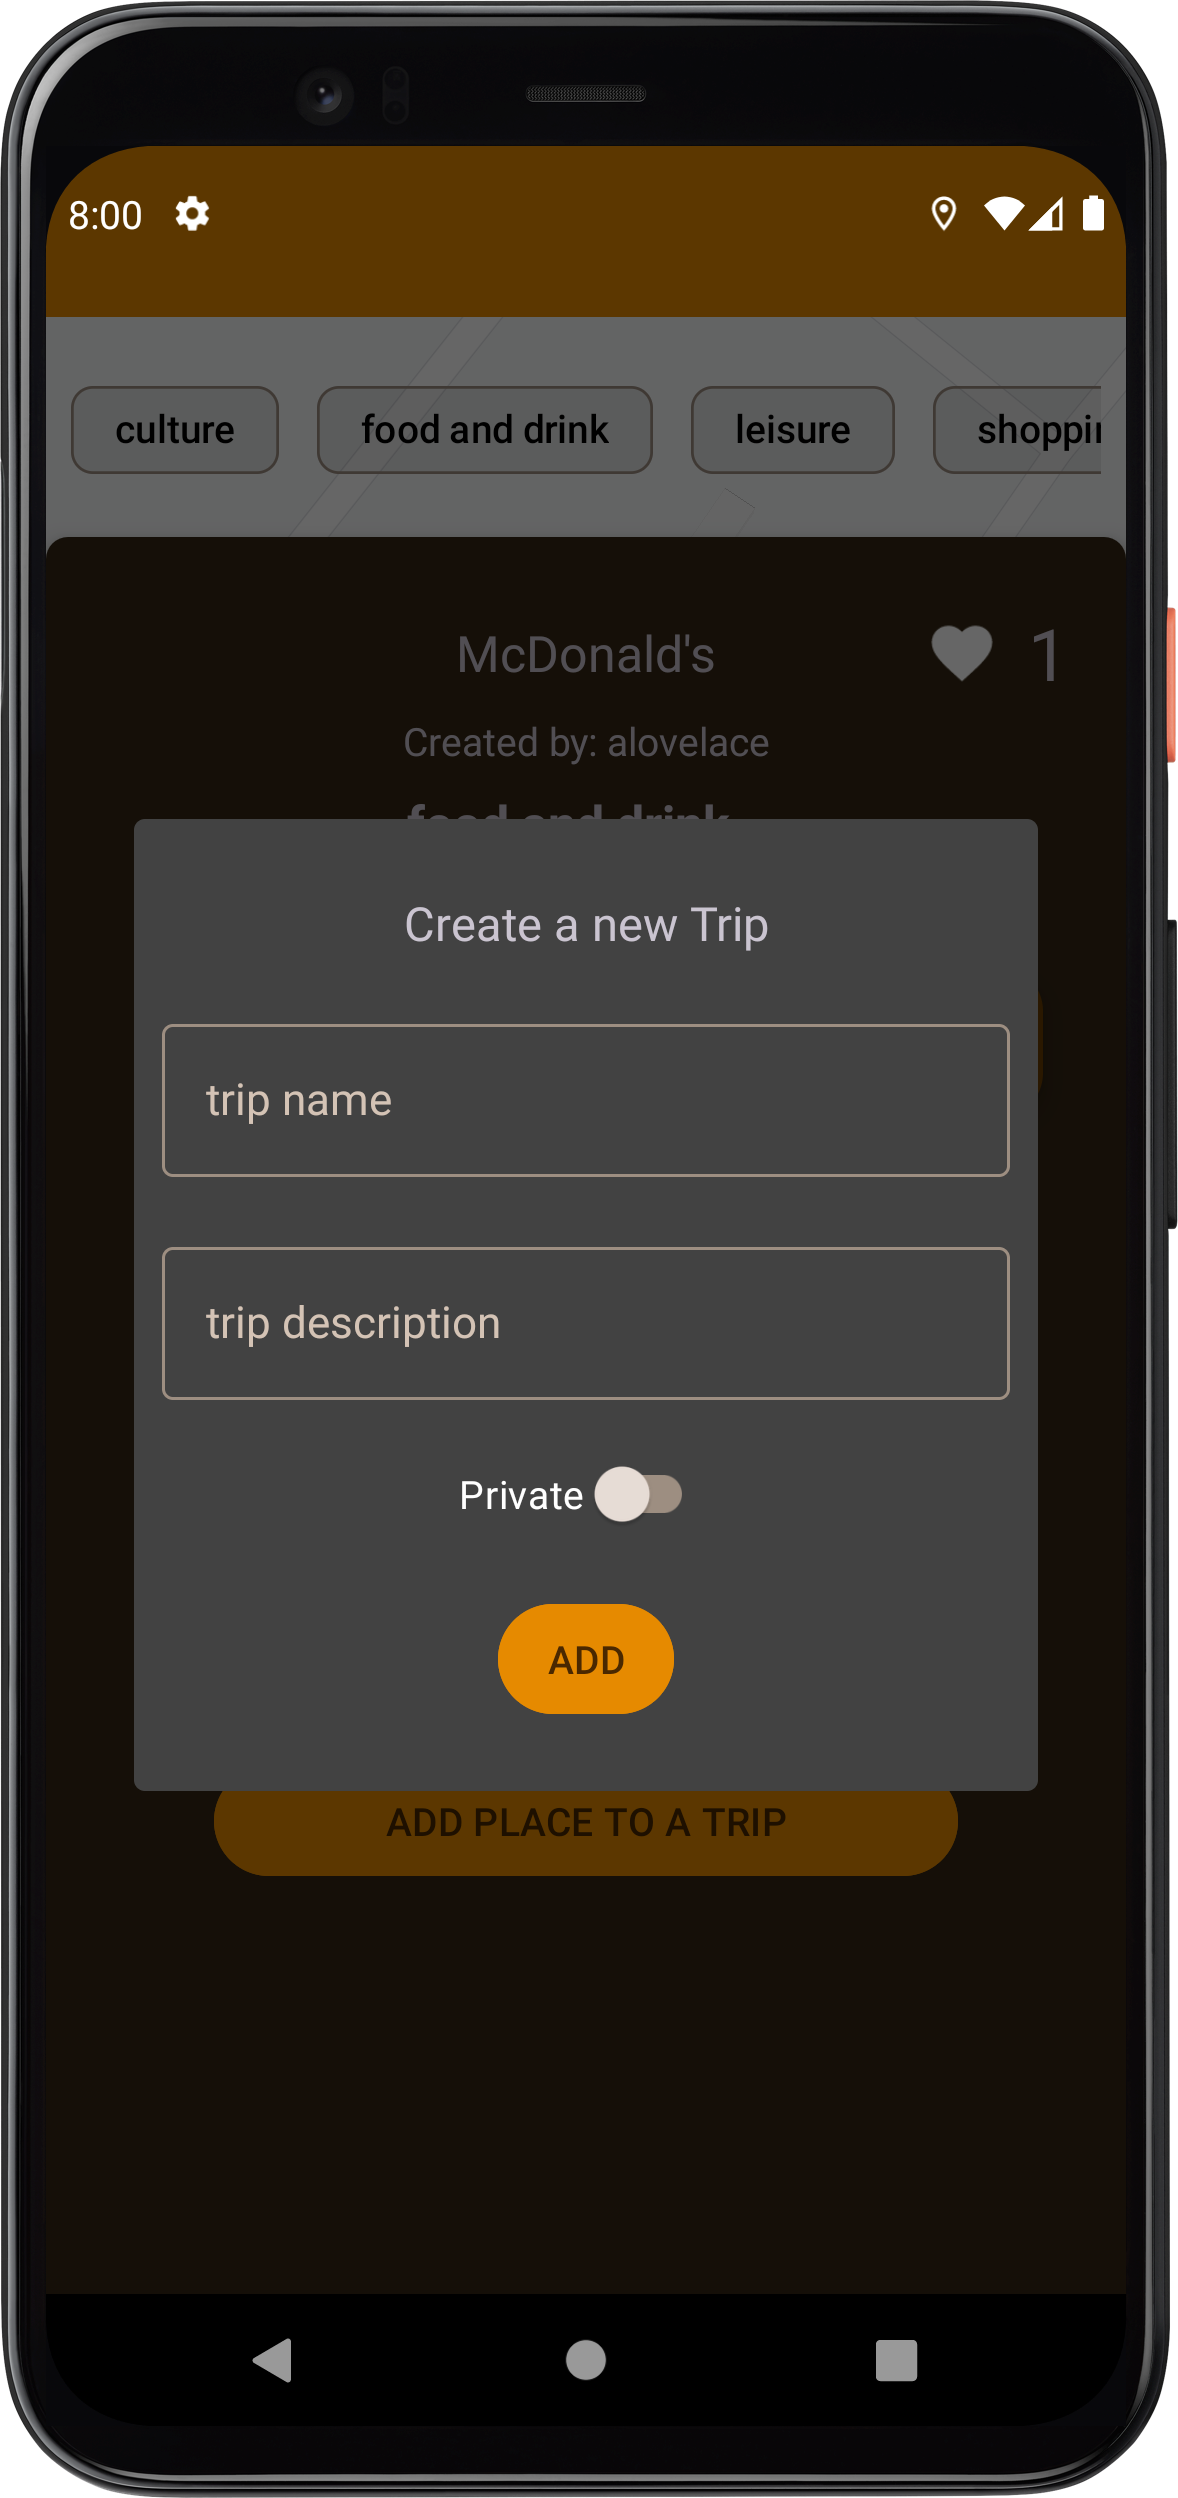
\includegraphics[width=\textwidth]{src/app/new_trip.png}
                \caption{Dialog tworzenia wycieczki.\label{trip_new}}
            \end{subfigure}
            \caption{Proces dodania miejsca do wycieczki.\label{trip}}
            \qquad
        \end{figure} 
        \vspace{1cm}

        \subsubsection{Ekran ustawień}
        Pierwszy od lewej przycisk na dolnym pasku kieruje użytkownika do ekranu ustawień. Znajduje się w nim jedynie opcja zmiany pseudonimu oraz opcja wylogowania się. Dzięki
        temu, że zmiany w Cloud Firestore zachodzą w czasie rzeczywistym, zmiana pseudonimu skutkuje w natychmiastowej zmianie nazwy autora widocznej m.in.\@ w arkuszu szczegółów miejsca.
        Przycisk wylogowania przenosi użytkownika do ekranu powitalnego. Ekran ustawień widoczny jest na rys.~\ref{settings}. Przy zmianie ekranu na inny niż ekran mapy zauważyć można, że
        przycisk dodania miejsca został zastąpiony przez przycisk przedstawiający kompas. Wciśnięcie go powoduje powrót do ekranu mapy.

        \vspace{1cm}
        \begin{figure}[H]
            \centering
            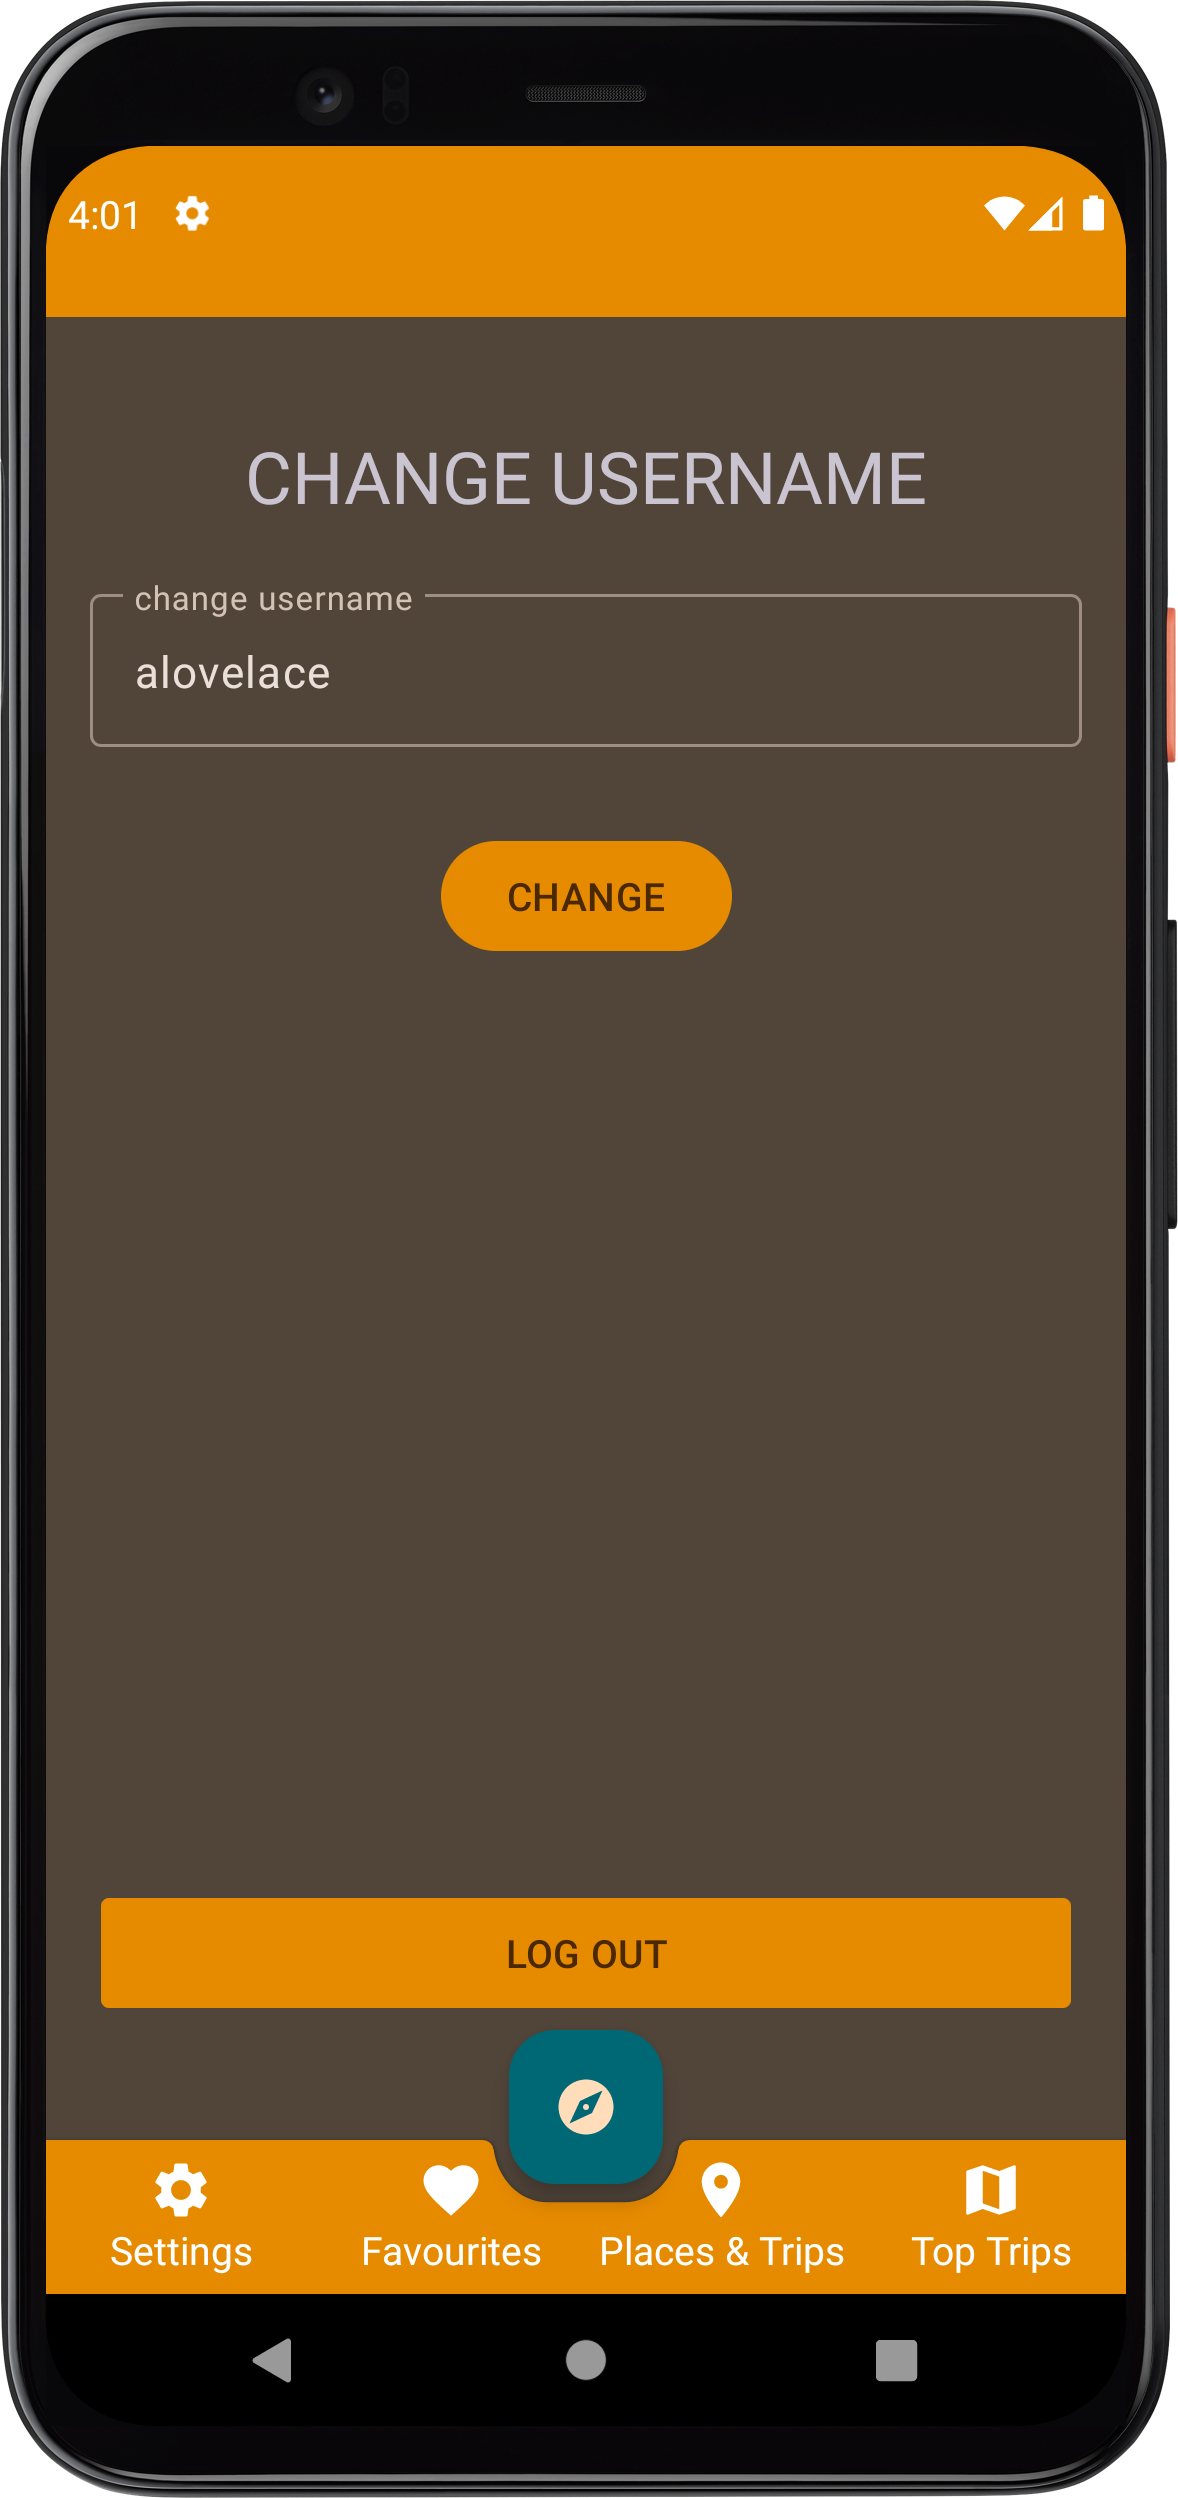
\includegraphics[scale=0.10]{src/app/settings.png}
            \caption{Widok ustawień.\label{settings}}
            \qquad
        \end{figure} 
        \vspace{1cm}

        \subsubsection{Listy ulubionych miejsc i wycieczek}
        Następny na pasku dolnym jest oznaczony kształtem serca przycisk zatytułowany „Favourites” (pol. Ulubione). Przekierowuje on użytkownika do ekranu, na którym wylistowane są polubione przez
        użytkownika miejsca oraz wycieczki. Znajdują się one na osobnych listach, które przełączać można, przesuwając palcem w prawo lub w lewo, zgodnie z wyświetlanymi na ekranie strzałkami.
        Na rys.~\ref{fav_place} zobaczyć można listę ulubionych miejsc użytkownika. Wciśnięcie elementu listy przeniesie użytkownika na ekran mapy i wyświetli na niej pinezkę tego miejsca.
        Wciśnięcie przycisku polubienia usunie miejsce z ulubionych i w czasie rzeczywistym zniknie z listy. Przesunięcie ekranu w lewo wyświetli listę ulubionych wycieczek widoczną na rys.~\ref{fav_trip1}.
        Każdy element listy posiada oznaczony strzałką przycisk rozwinięcia pozwalający zobaczyć podgląd opisu danej wycieczki, co widoczne jest na rys.~\ref{fav_trip2}.
        
        \vspace{1cm}
        \begin{figure}[H]
            \centering
            \begin{subfigure}[b]{0.3\textwidth}
                \centering
                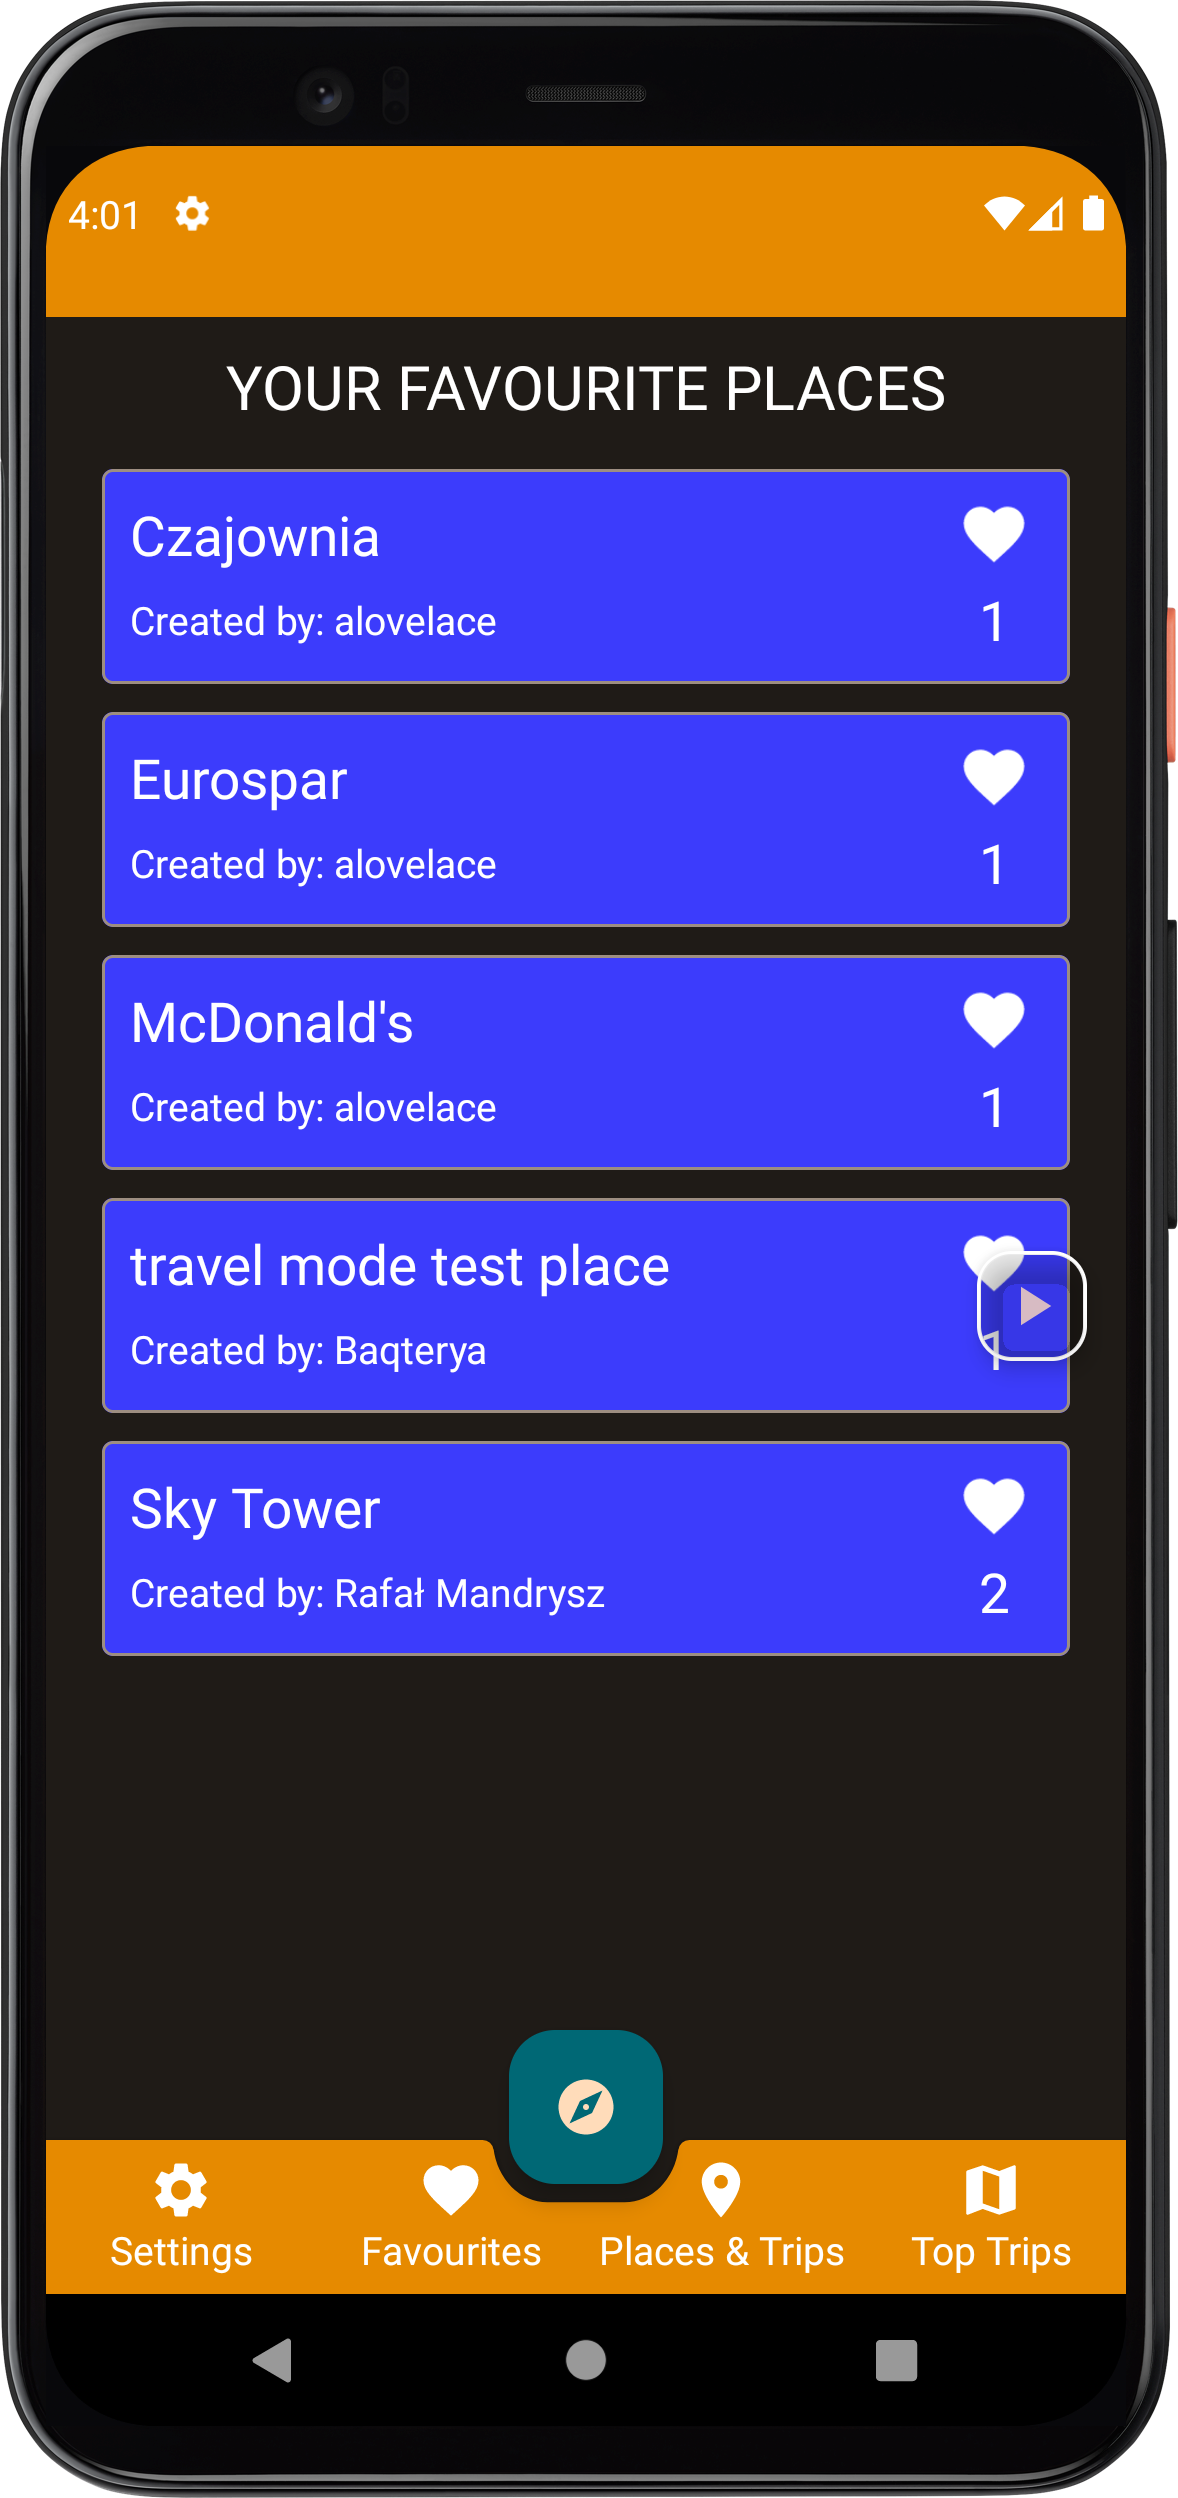
\includegraphics[width=\textwidth]{src/app/fav_places.png}
                \caption{Lista ulubionych miejsc użytkownika.\label{fav_place}}
            \end{subfigure}
            \hfill
            \begin{subfigure}[b]{0.3\textwidth}
                \centering
                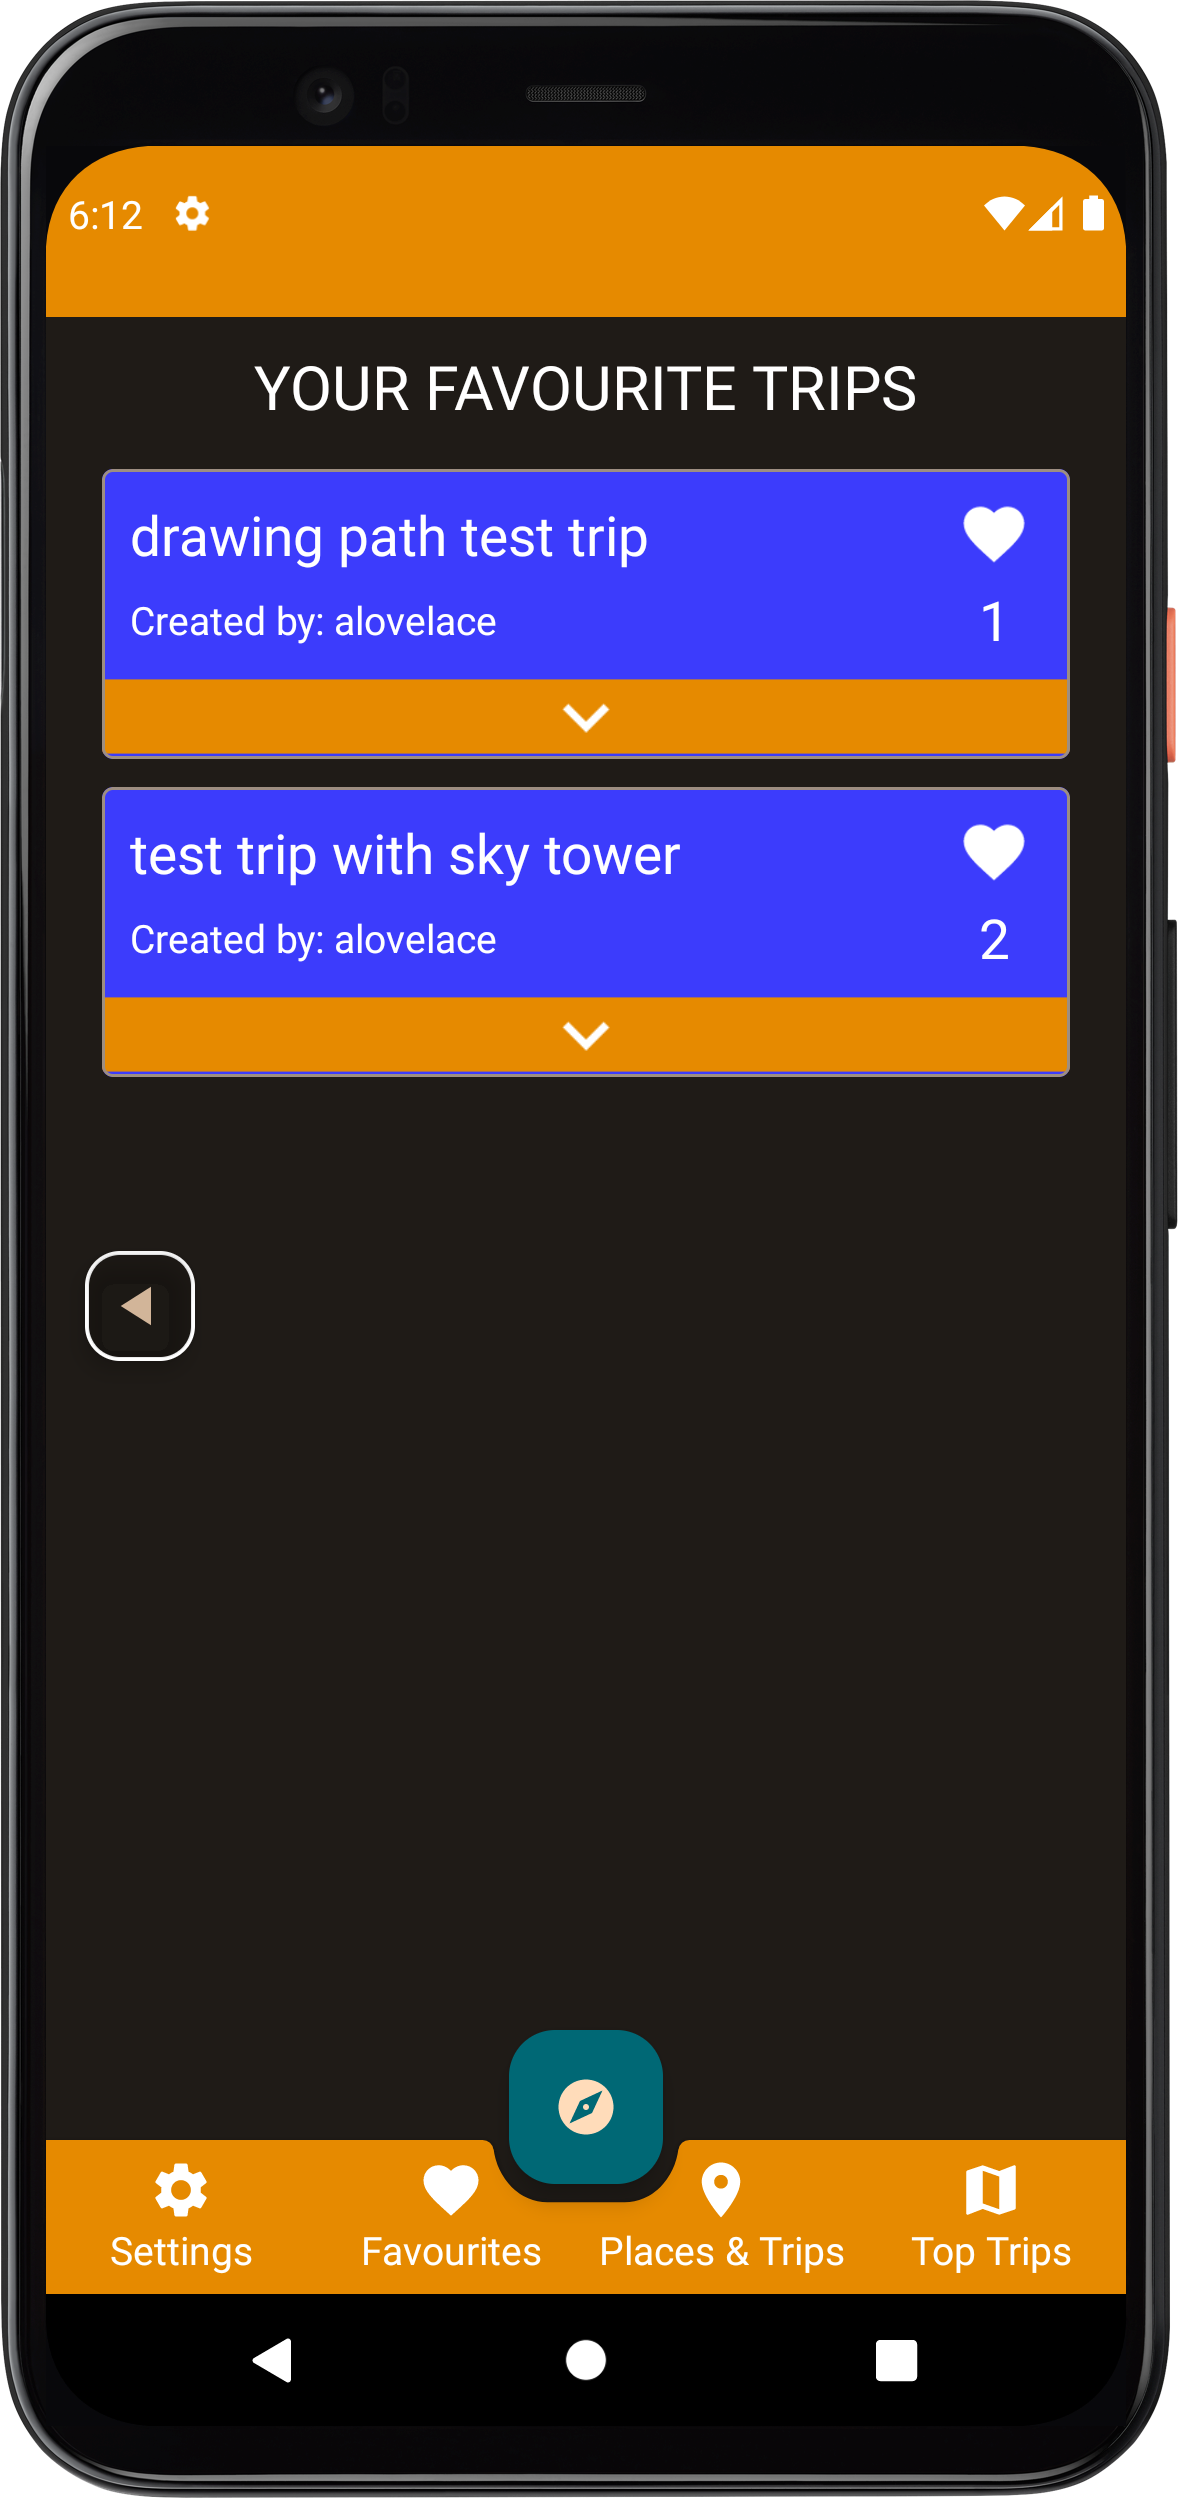
\includegraphics[width=\textwidth]{src/app/fav_trips1.png}
                \caption{Lista ulubionych wycieczek.\label{fav_trip1}}
            \end{subfigure}
            \hfill
            \begin{subfigure}[b]{0.3\textwidth}
                \centering
                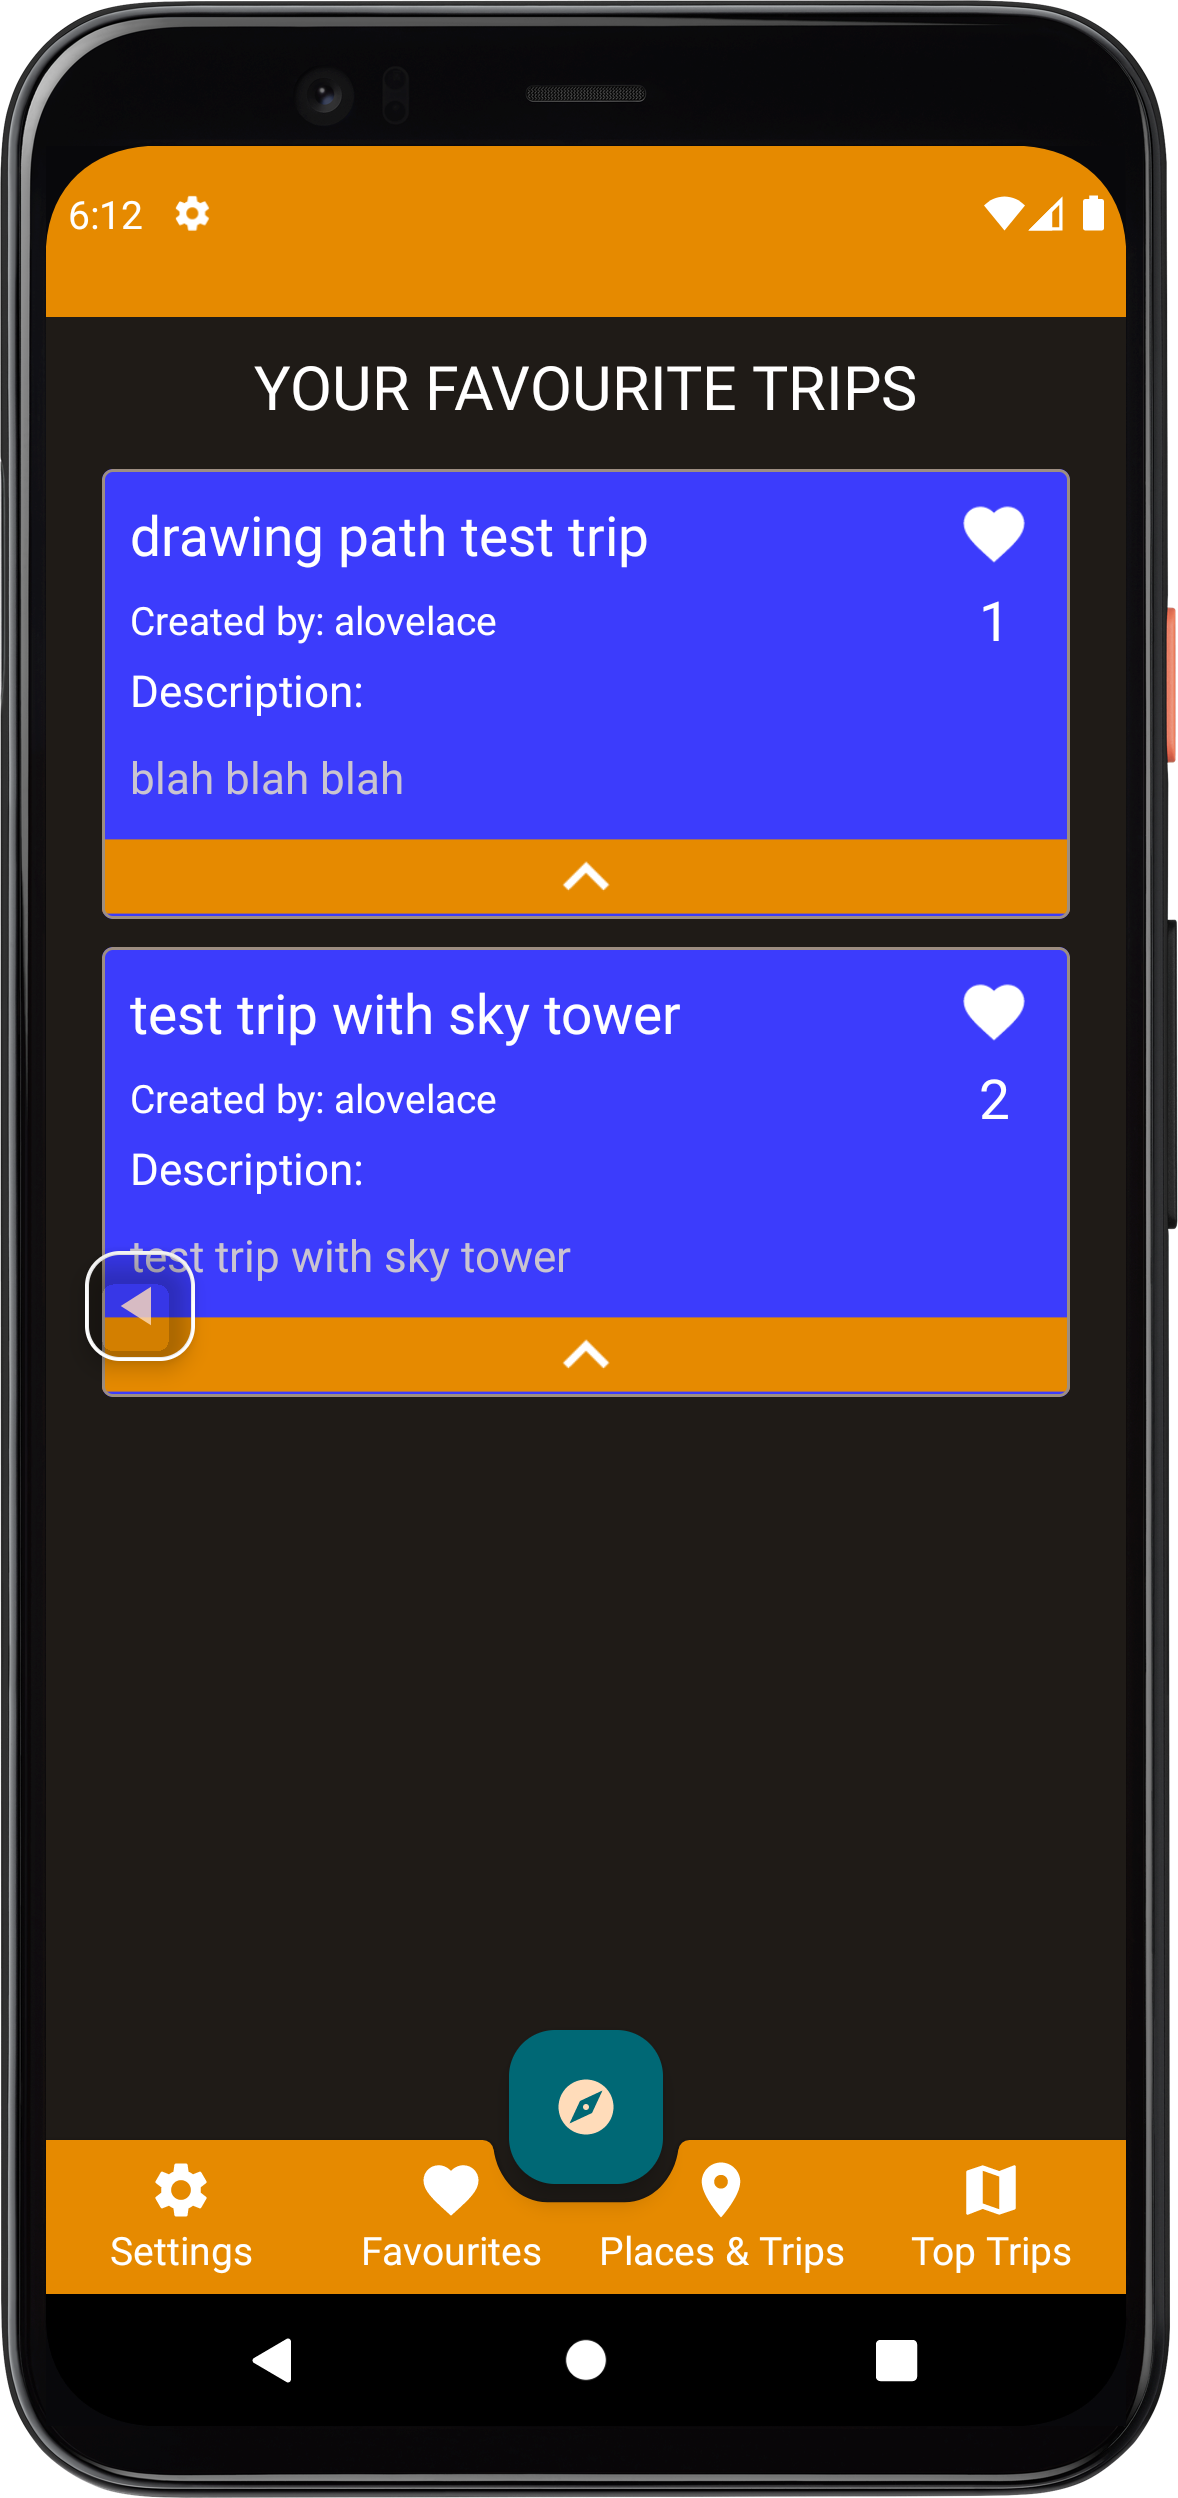
\includegraphics[width=\textwidth]{src/app/fav_trips2.png}
                \caption{Rozwinięty opis wycieczek.\label{fav_trip2}}
            \end{subfigure}
            \caption{Ekran ulubionych miejsc i wycieczek.\label{fav}}
            \qquad
        \end{figure} 
        \vspace{1cm}
        
        Wciśnięcie elementu listy wycieczek przeniesie użytkownika do widocznego na rys~\ref{trip_det} ekranu szczegółów wycieczki. Na samej górze ekranu widoczna jest nazwa wycieczki.
        Pod nią mieszczą się pseudonim autora, opis oraz lista miejsc zawierających się w wycieczce. Wciśnięcie elementu listy miejsc przekieruje użytkownika do ekranu mapy i wyświetli na niej
        pinezkę przedstawiającą wybrane miejsce.

        \vspace{1cm}
        \begin{figure}[H]
            \centering
            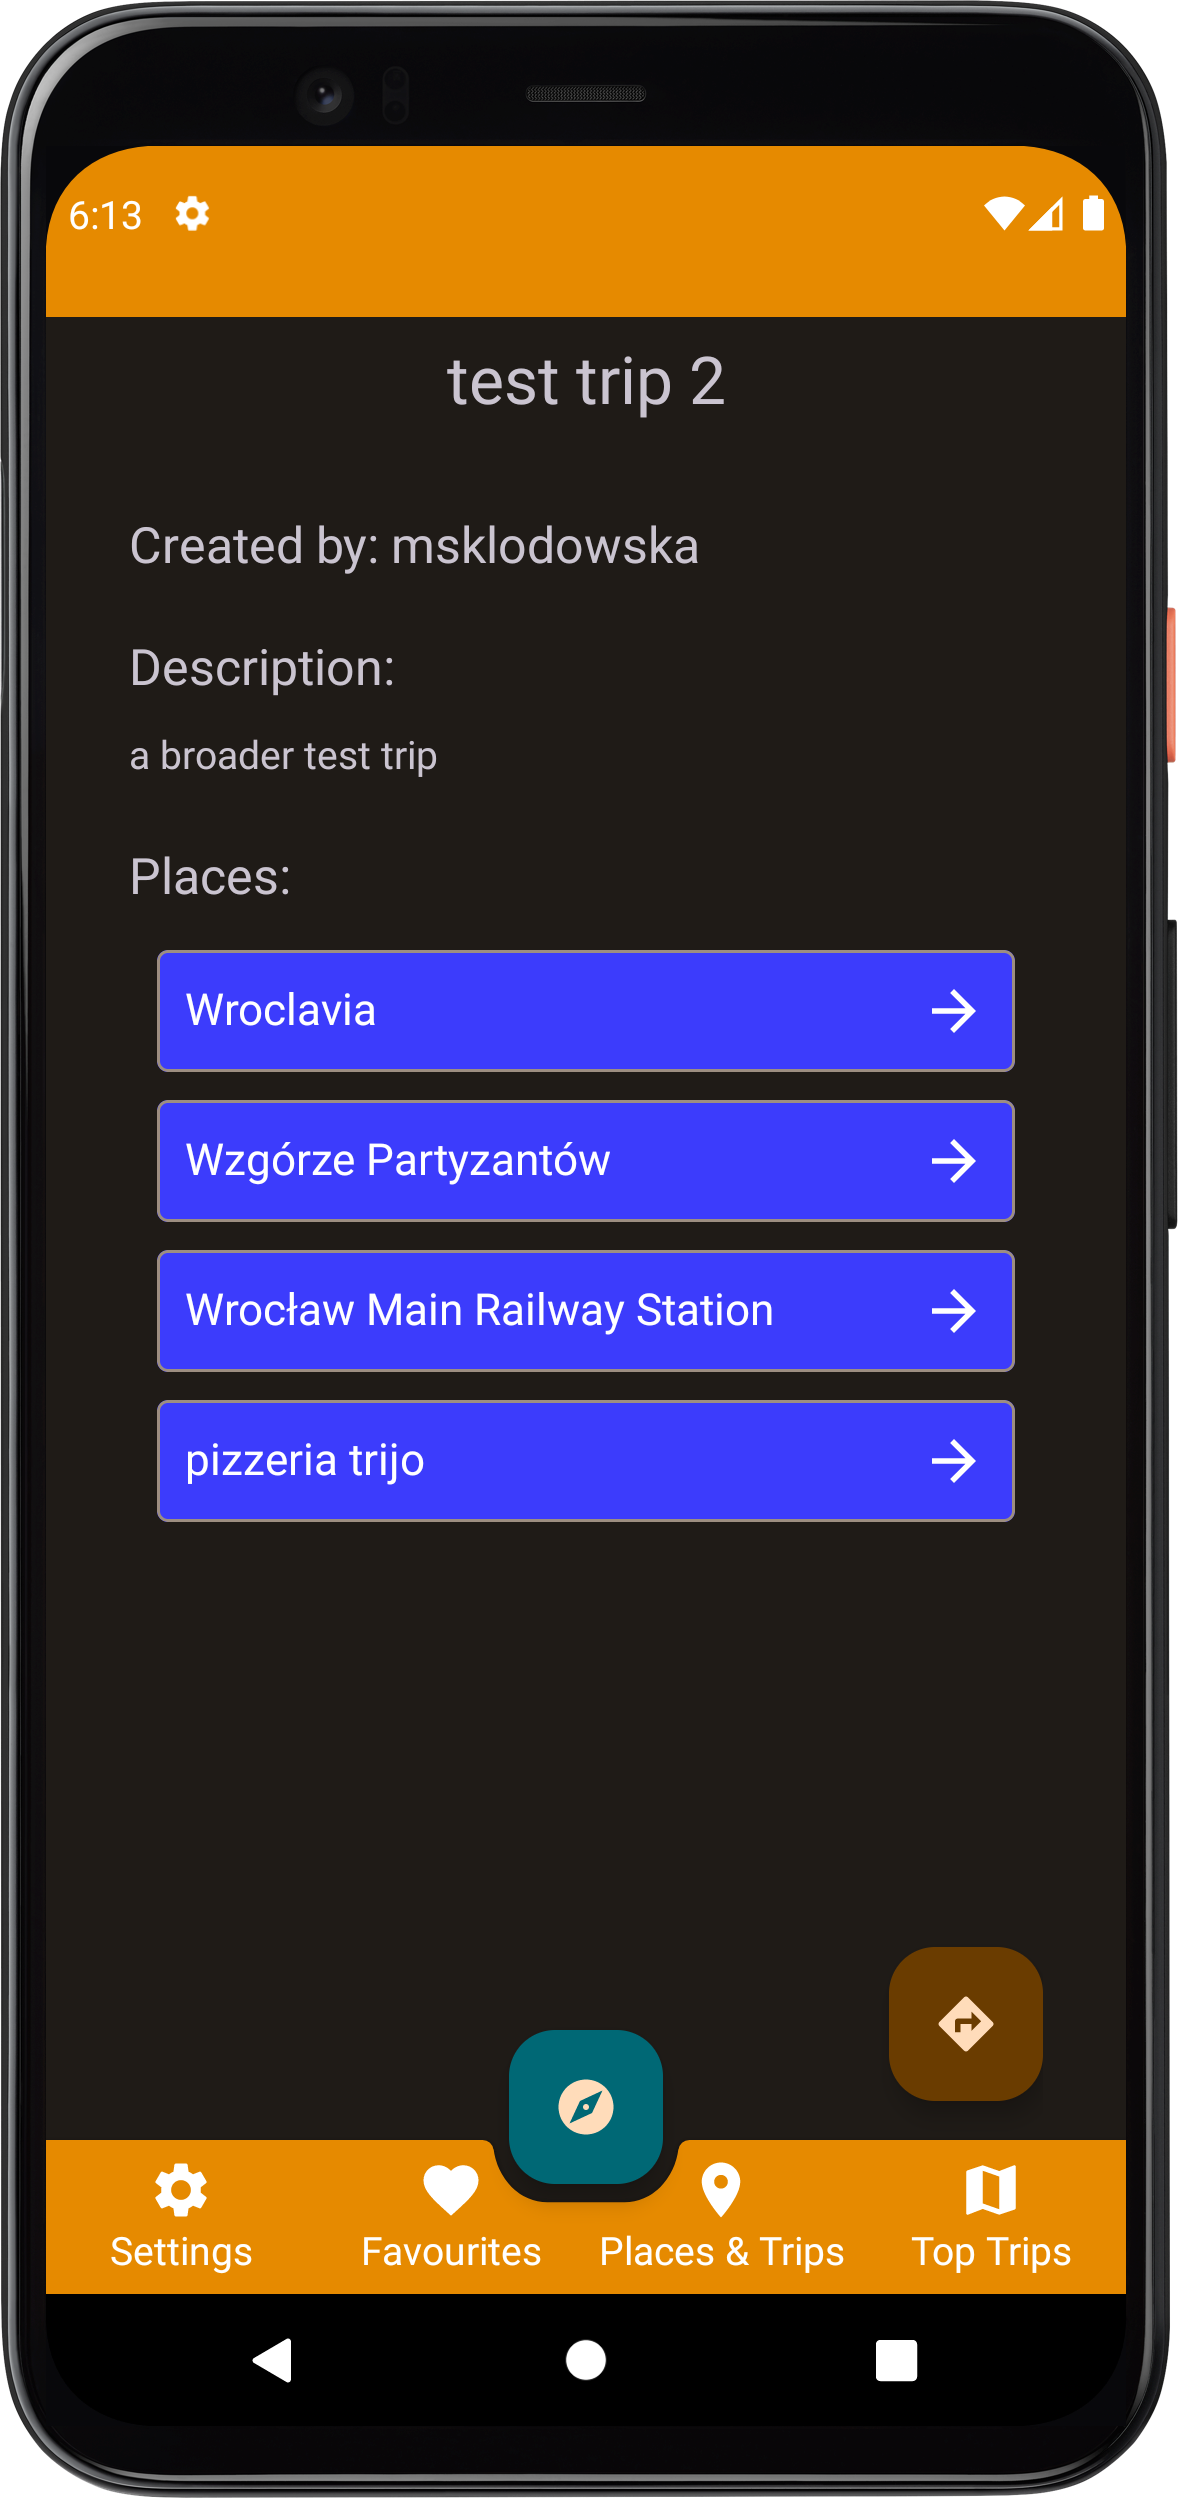
\includegraphics[scale=0.10]{src/app/trip.png}
            \caption{Ekran szczegółów wycieczki.\label{trip_det}}
            \qquad
        \end{figure} 
        \vspace{1cm}

        W prawym dole ekranu szczegółów wycieczki widoczny jest oznaczony znakiem drogowym przycisk rysowania trasy wycieczki. Przekierowuje on użytkownika na ekran mapy, gdzie zaczyna się proces 
        rysowania trasy. Rozpoczyna się ona w aktualnej pozycji użytkownika, a kończy w ostatnim miejscu na liście. Po przekierowaniu na ekranie widoczny jest dolny arkusz pozwalający użytkownikowi
        na wybór pomiędzy pieszą a samochodową trasą oraz lista miejsc. Pozycje na liście oznaczone są ikoną mającą sugerować użytkownikowi, że może zmieniać kolejność elementów na liście,
        wybierając w ten sposób kolejność odwiedzania miejsc wycieczki. Widok ten przedstawiony jest na rys.~\ref{draw}.

        \vspace{1cm}
        \begin{figure}[H]
            \centering
            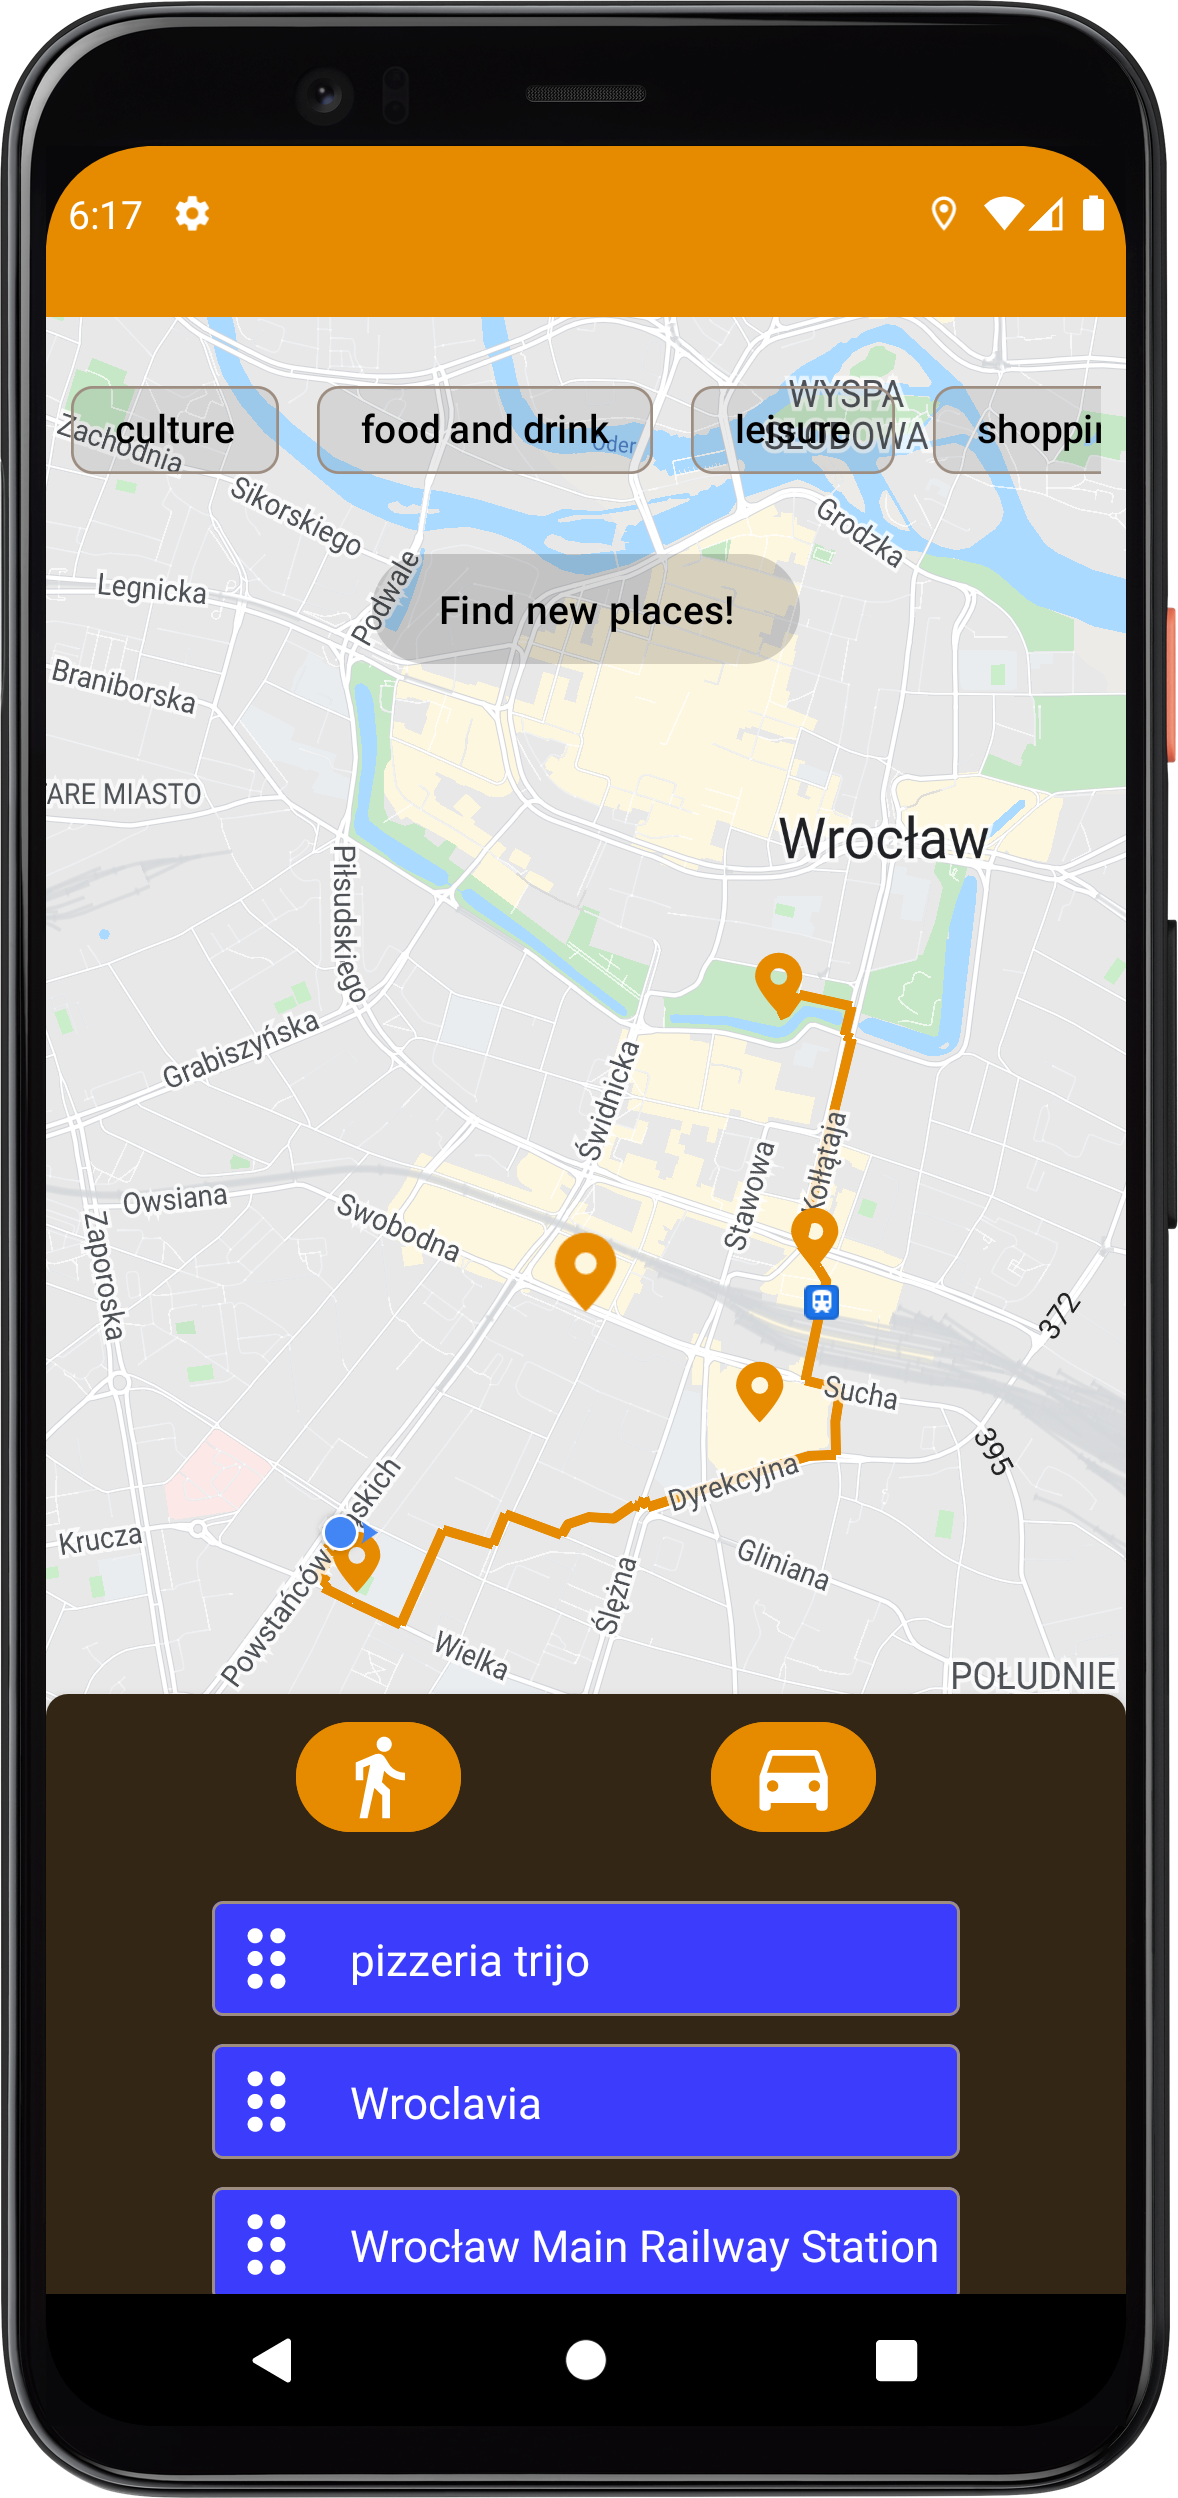
\includegraphics[scale=0.10]{src/app/drawing_trip.png}
            \caption{Proces planowania trasy wycieczki.\label{draw}}
            \qquad
        \end{figure} 
        \vspace{1cm}

        \subsubsection{Listy miejsc i wycieczek użytkownika}
        Trzecia z opcji widocznych na pasku dolnym opisana jest „Places and Trips” i przedstawia ona listy miejsc i wycieczek stworzonych przez użytkownika. Ekran ten widoczny jest na rys.~\ref{user_stuff}.
        Poruszanie się pomiędzy listą miejsc i wycieczek działa w ten sam sposób, co w opisanym wcześniej ekranie „Favourites”. Widoczna na rys.~\ref{user_places} lista przedstawia wszystkie dodane
        przez użytkownika miejsca wraz z liczbą ich polubień przez wszystkich użytkowników. Podobnie skonstruowana jest widoczna na rys.~\ref{user_trips} lista wycieczek stworzonych przez użytkownika.

        \vspace{1cm}
        \begin{figure}[H]
            \centering
            \begin{subfigure}[b]{0.3\textwidth}
                \centering
                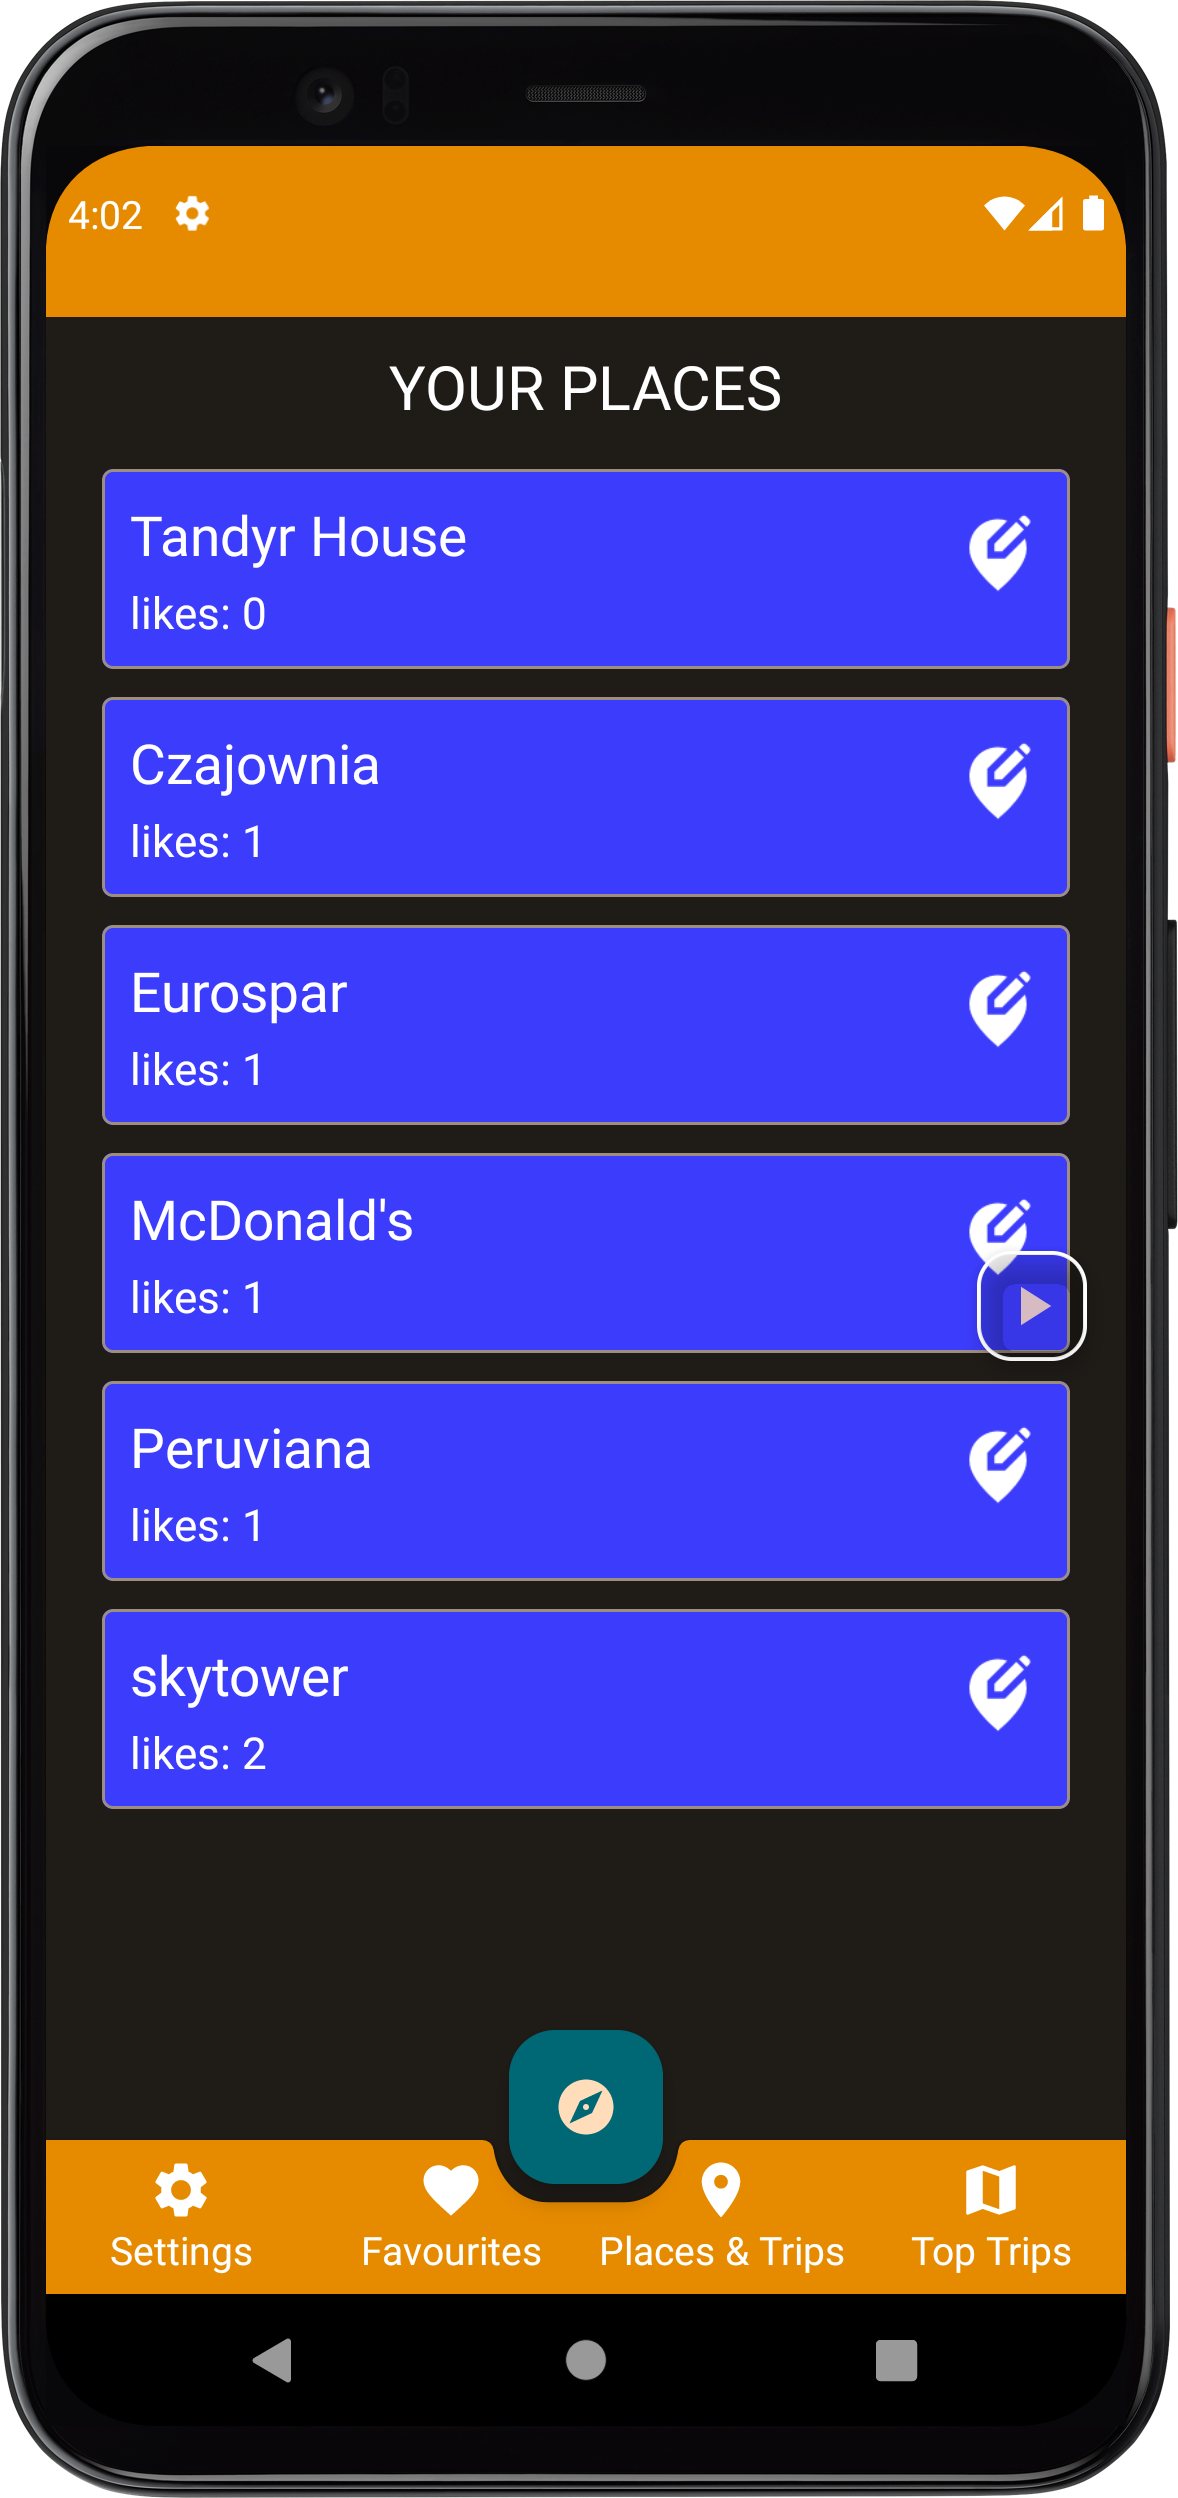
\includegraphics[width=\textwidth]{src/app/user_places.png}
                \caption{Lista miejsc użytkownika.\label{user_places}}
            \end{subfigure}
            \hfill
            \begin{subfigure}[b]{0.3\textwidth}
                \centering
                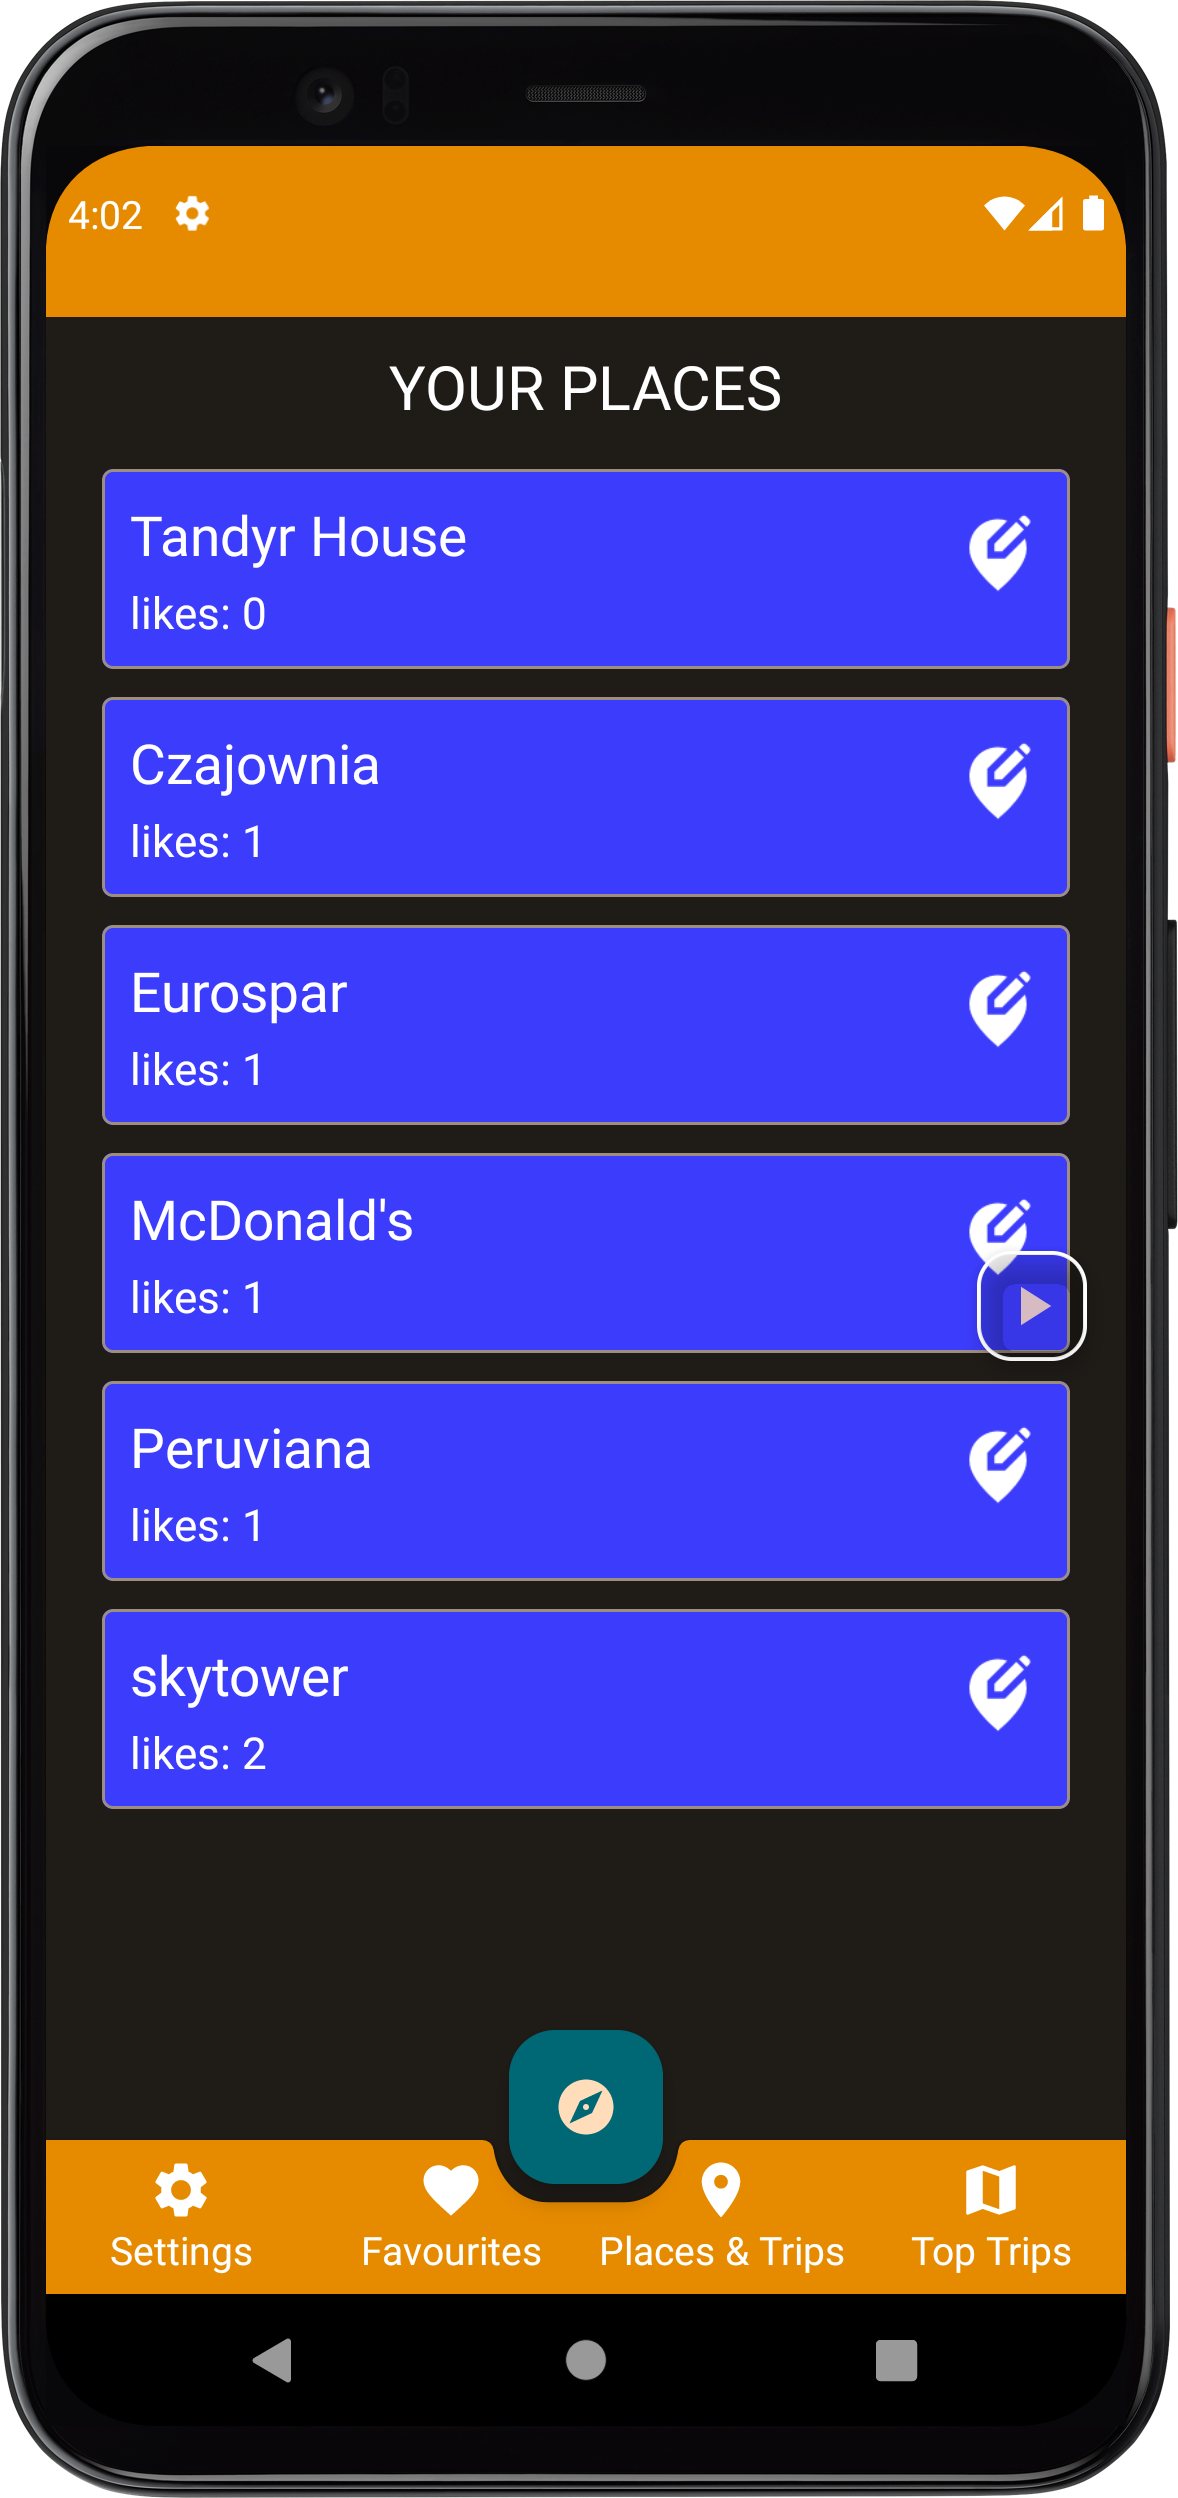
\includegraphics[width=\textwidth]{src/app/user_places.png}
                \caption{Lista wycieczek użytkownika.\label{user_trips}}
            \end{subfigure}
            \caption{Ekran miejsc i wycieczek użytkownika.\label{user_stuff}}
            \qquad
        \end{figure} 
        \vspace{1cm}

        Wciśnięcie elementu listy miejsc stworzonych przez użytkownika przekierowuje użytkownika do ekranu mapy, na której wyświetlone zostaje wybrane miejsce.
        Wciśnięcie ikony edycji miejsca skutkuje wyświetleniem dialogu edycji miejsca widocznego na rys.~\ref{edit_place}. Jest on analogiczny do przedstawionego wcześniej 
        ekranu dialogowego służącego do utworzenia miejsca, z tą różnicą, że jest on uzupełniony aktualnymi danymi miejsca oraz obok nazwy miejsca widoczny jest 
        przedstawiający ikonę kosza przycisk usunięcia miejsca. Powoduje on, poprzedzone dialogiem ostrzegawczym, bezpowrotne usunięcie miejsca z bazy danych.
        Znajdujący się na dole ekranu dialogowego przycisk „Save” (pol. Zapisz) zapisuje zmiany wprowadzone przez użytkownika. Wciśnięcie elementu listy wycieczek
        użytkownika przenosi użytkownika do ekranu edycji wycieczki. Widoczne są w nim pola do edycji nazwy, opisu i prywatności wycieczki, przycisk usunięcia, działający
        jednakowo do przycisku usunięcia miejsca, oraz lista zawartych w wycieczce miejsc. Elementy listy miejsc wycieczki opatrzone są ikoną „X”, której wciśnięcie
        skutkuje usunięciem miejsca z wycieczki. Ekran edycji wycieczki przedstawiony jest na rys.~\ref{edit_trip}.

        \vspace{1cm}
        \begin{figure}[H]
            \centering
            \begin{subfigure}[b]{0.3\textwidth}
                \centering
                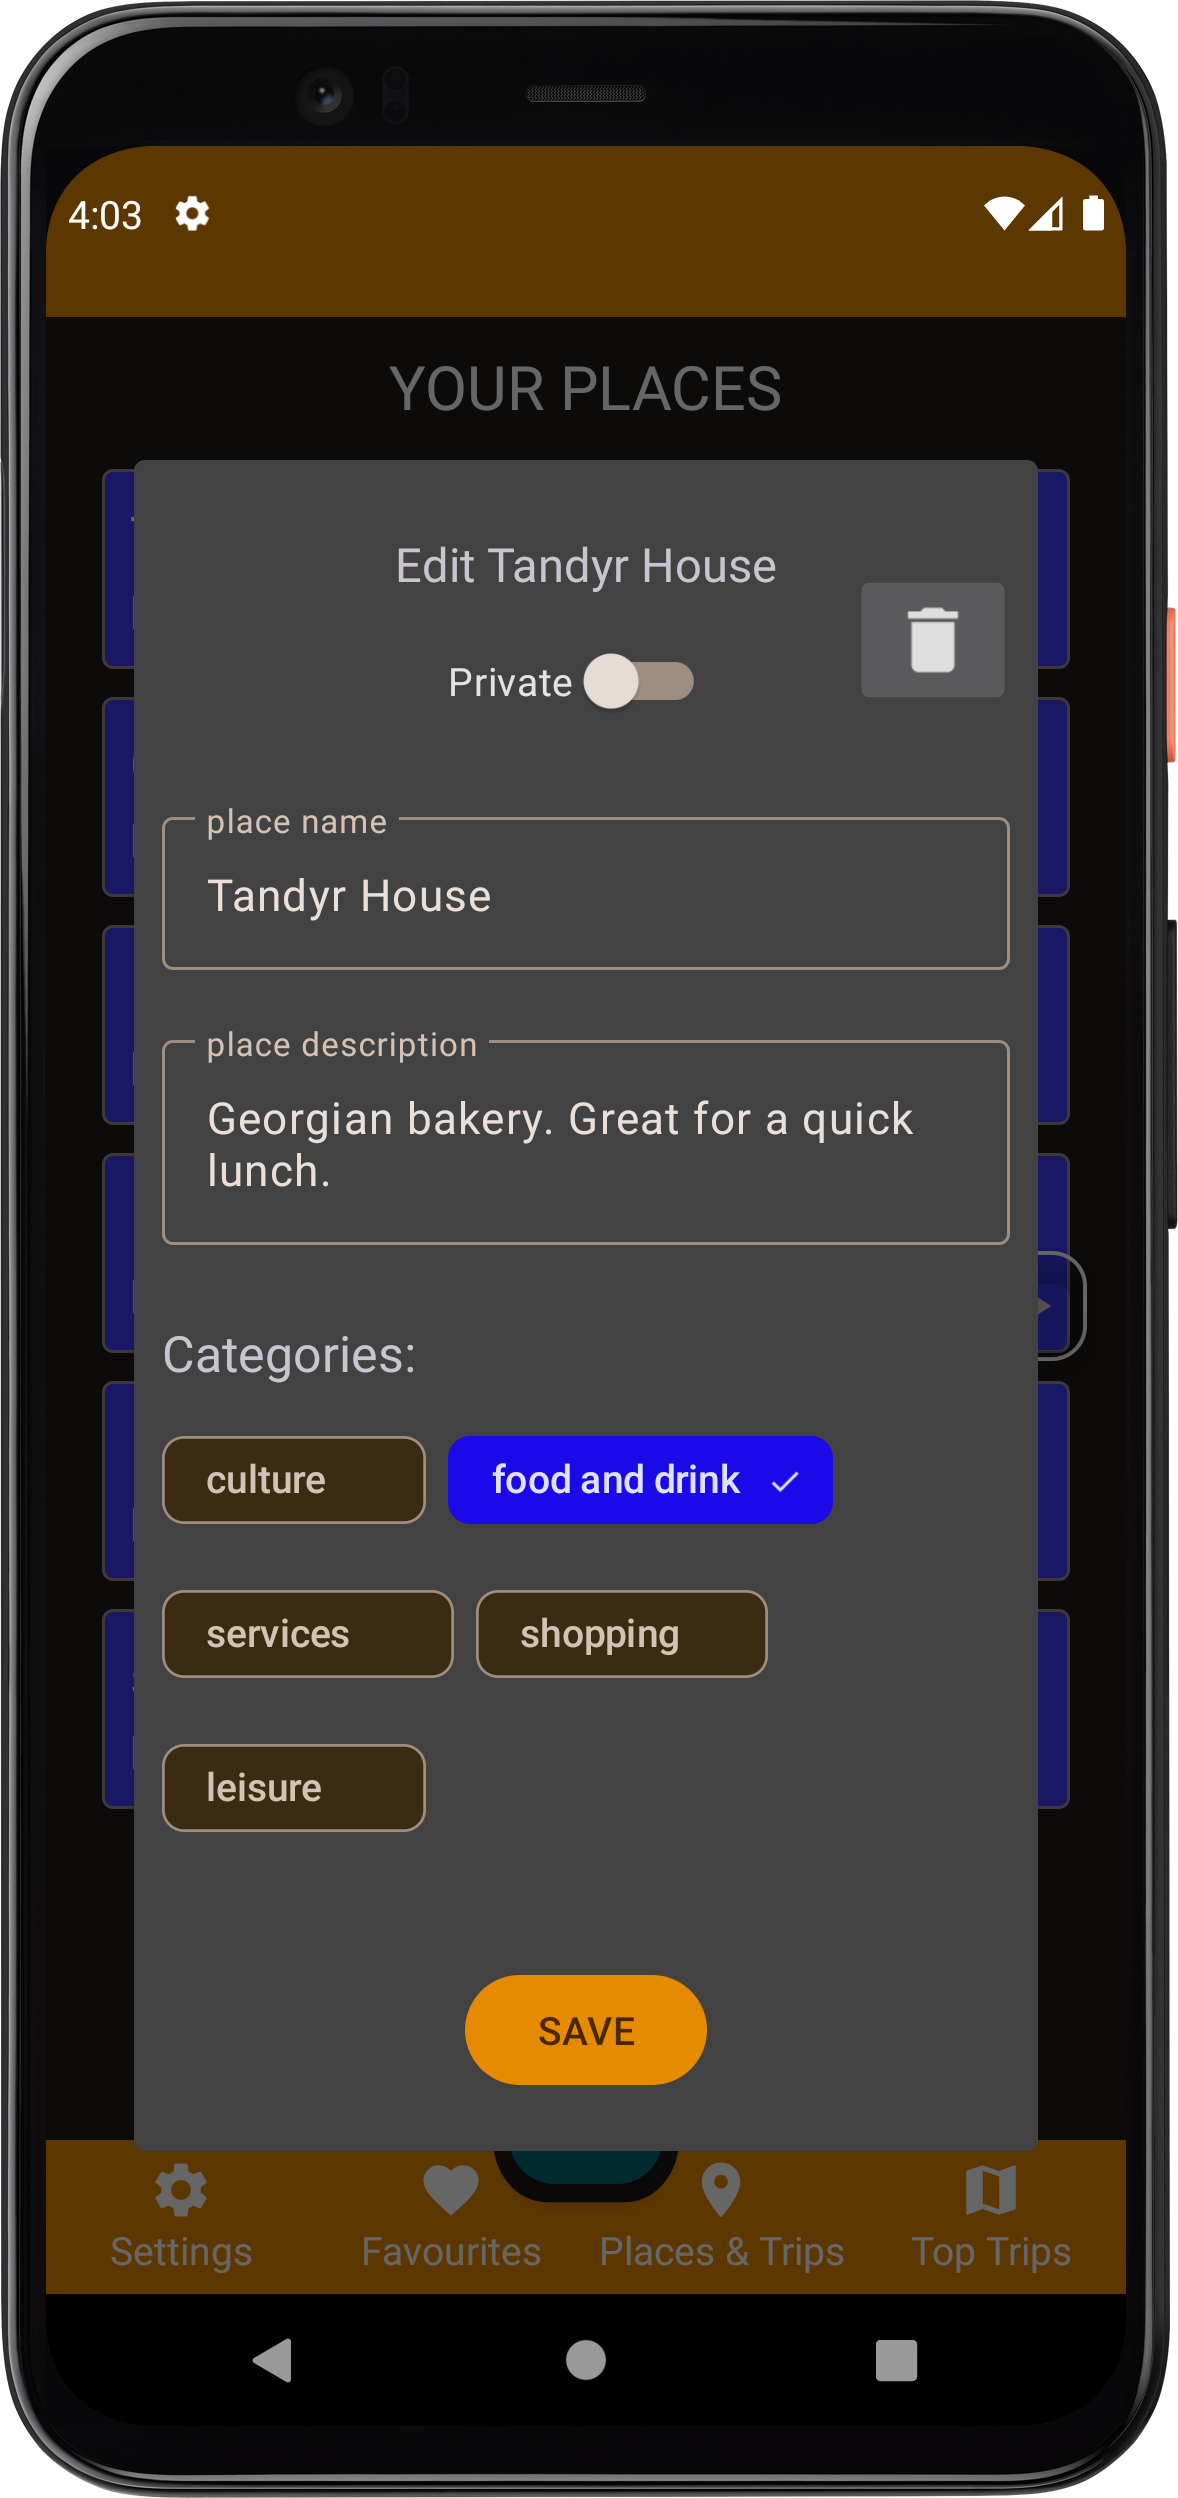
\includegraphics[width=\textwidth]{src/app/edit_place.png}
                \caption{Dialog edycji miejsca.\label{edit_place}}
            \end{subfigure}
            \hfill
            \begin{subfigure}[b]{0.3\textwidth}
                \centering
                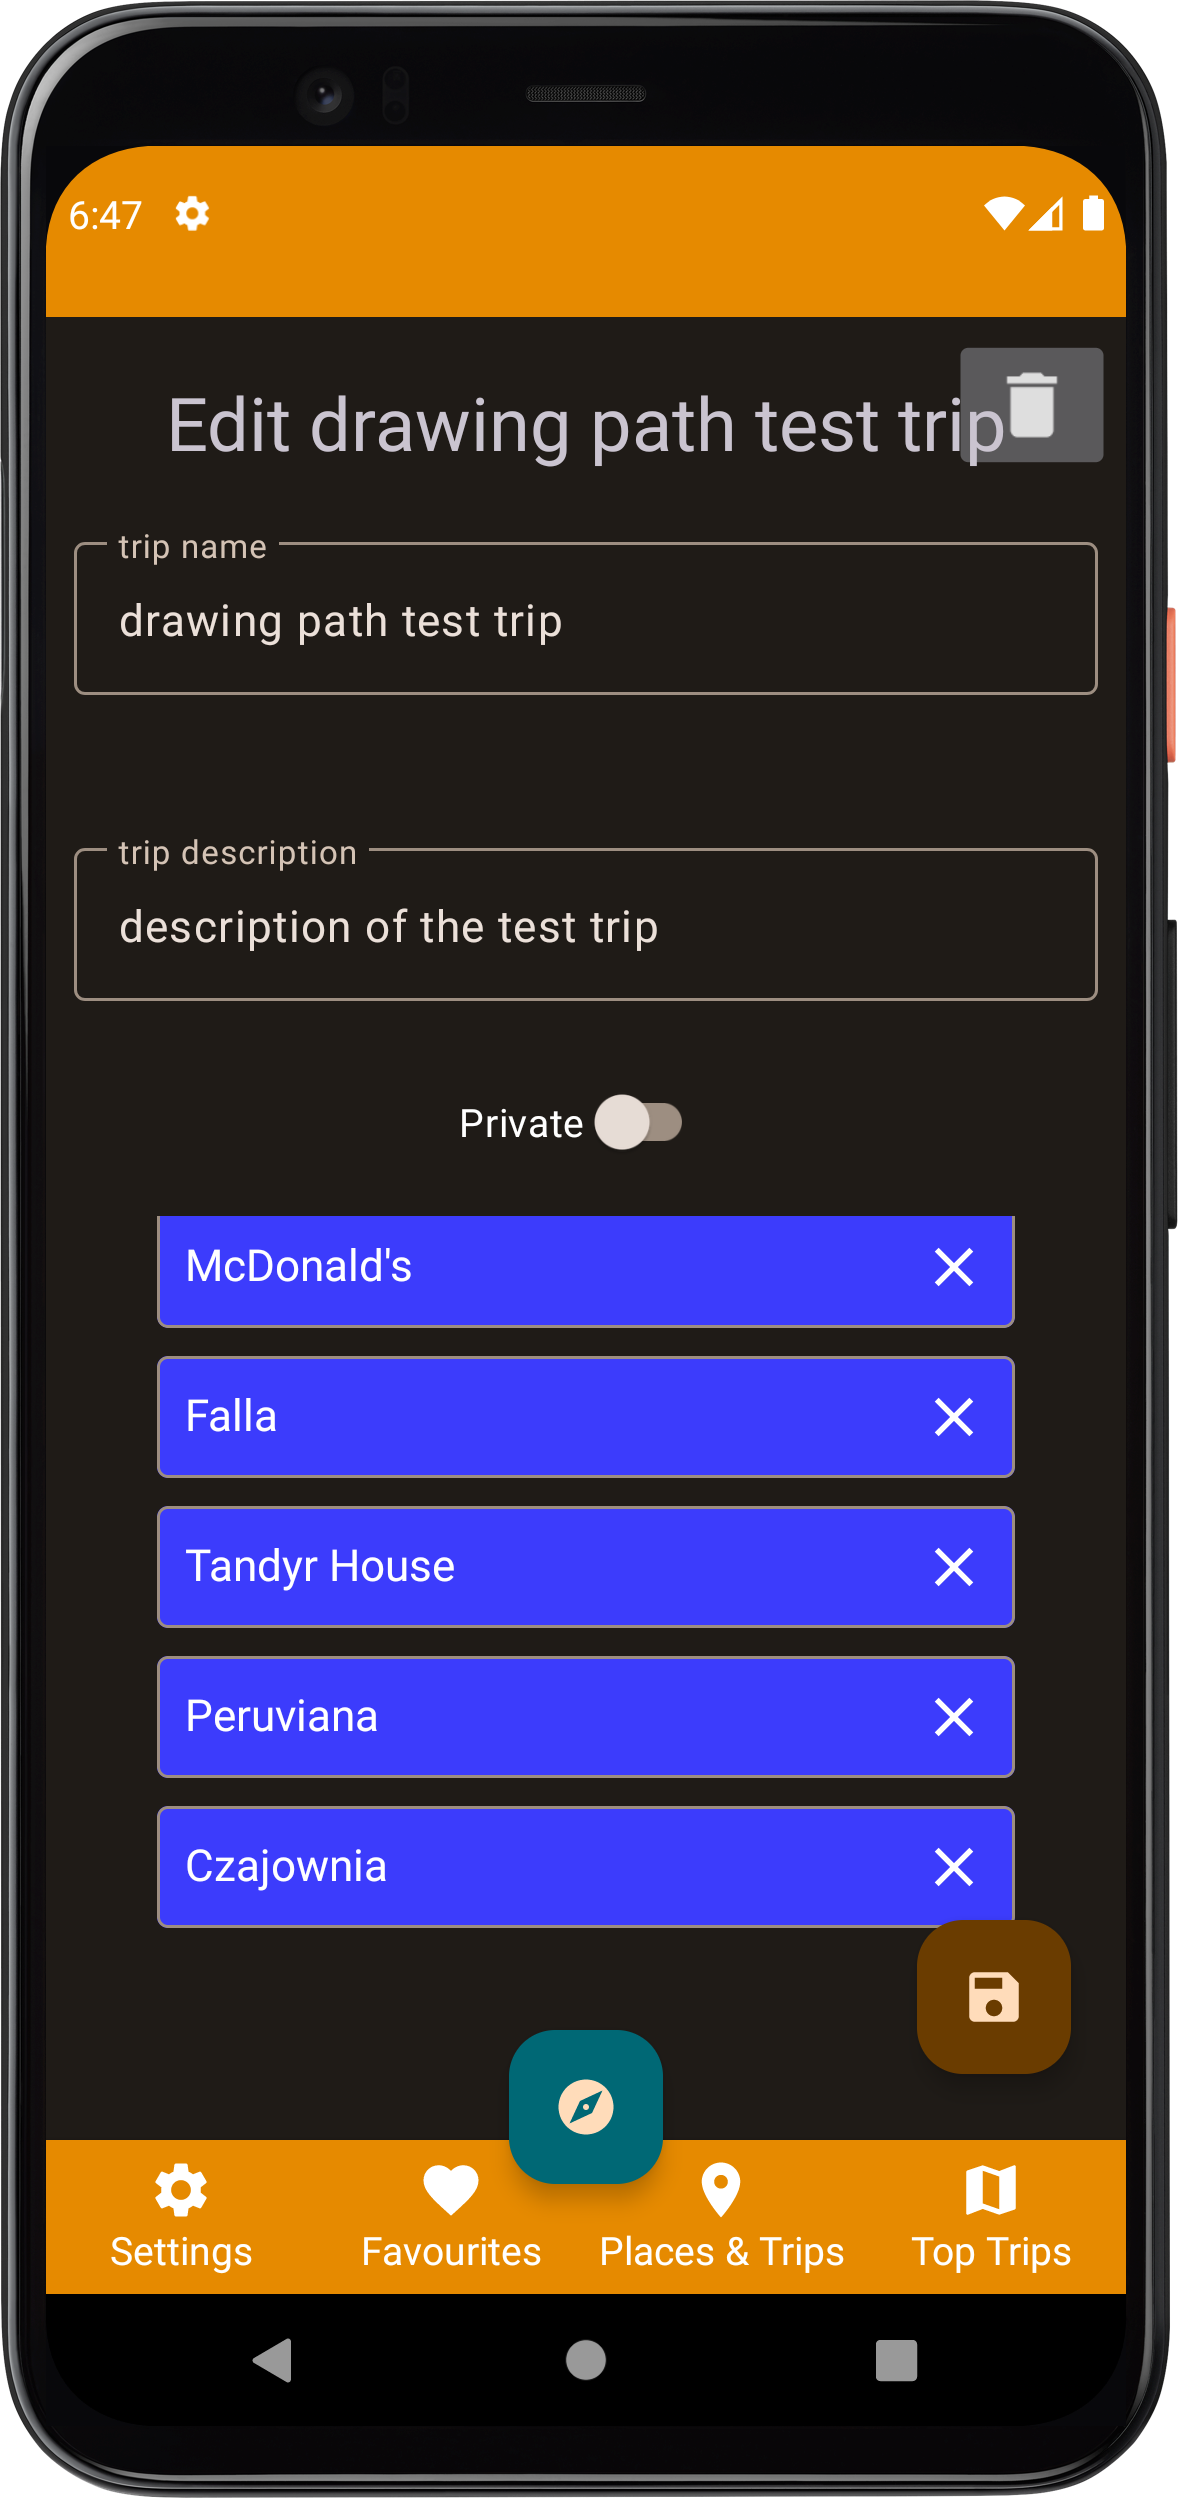
\includegraphics[width=\textwidth]{src/app/edit_trip.png}
                \caption{Ekran edycji wycieczki.\label{edit_trip}}
            \end{subfigure}
            \caption{Edycja miejsc i wycieczek użytkownika.\label{edit}}
            \qquad
        \end{figure} 
        \vspace{1cm}

        \subsubsection{Lista najpopularniejszych wycieczek}
        Ostatni z dostępnych w aplikacji ekranów to ekran przedstawiający listę stu nieprywatnych wycieczek stworzonych przez użytkowników aplikacji o największej ilości polubień. 
        Są one posortowane względem polubień. Jest to sposób na to, aby użytkownicy mogli odkrywać stworzone przez innych wycieczki i poznawać popularne trasy. Elementy 
        listy przedstawiają nazwę, twórcę oraz ilość polubień wycieczek, oraz przycisk pozwalający rozwinąć ich opis. Wciśnięcie przycisku polubienia doda miejsce do ulubionych miejsc
        użytkownika. Wciśnięcie elementu listy przeniesie użytkownika do widocznego na rys.~\ref{trip} ekranu szczegółów miejsca. Ekran listy najpopularniejszych wycieczek widoczny jest 
        na rys.~\ref{top_trips}.

        \vspace{1cm}
        \begin{figure}[H]
            \centering
            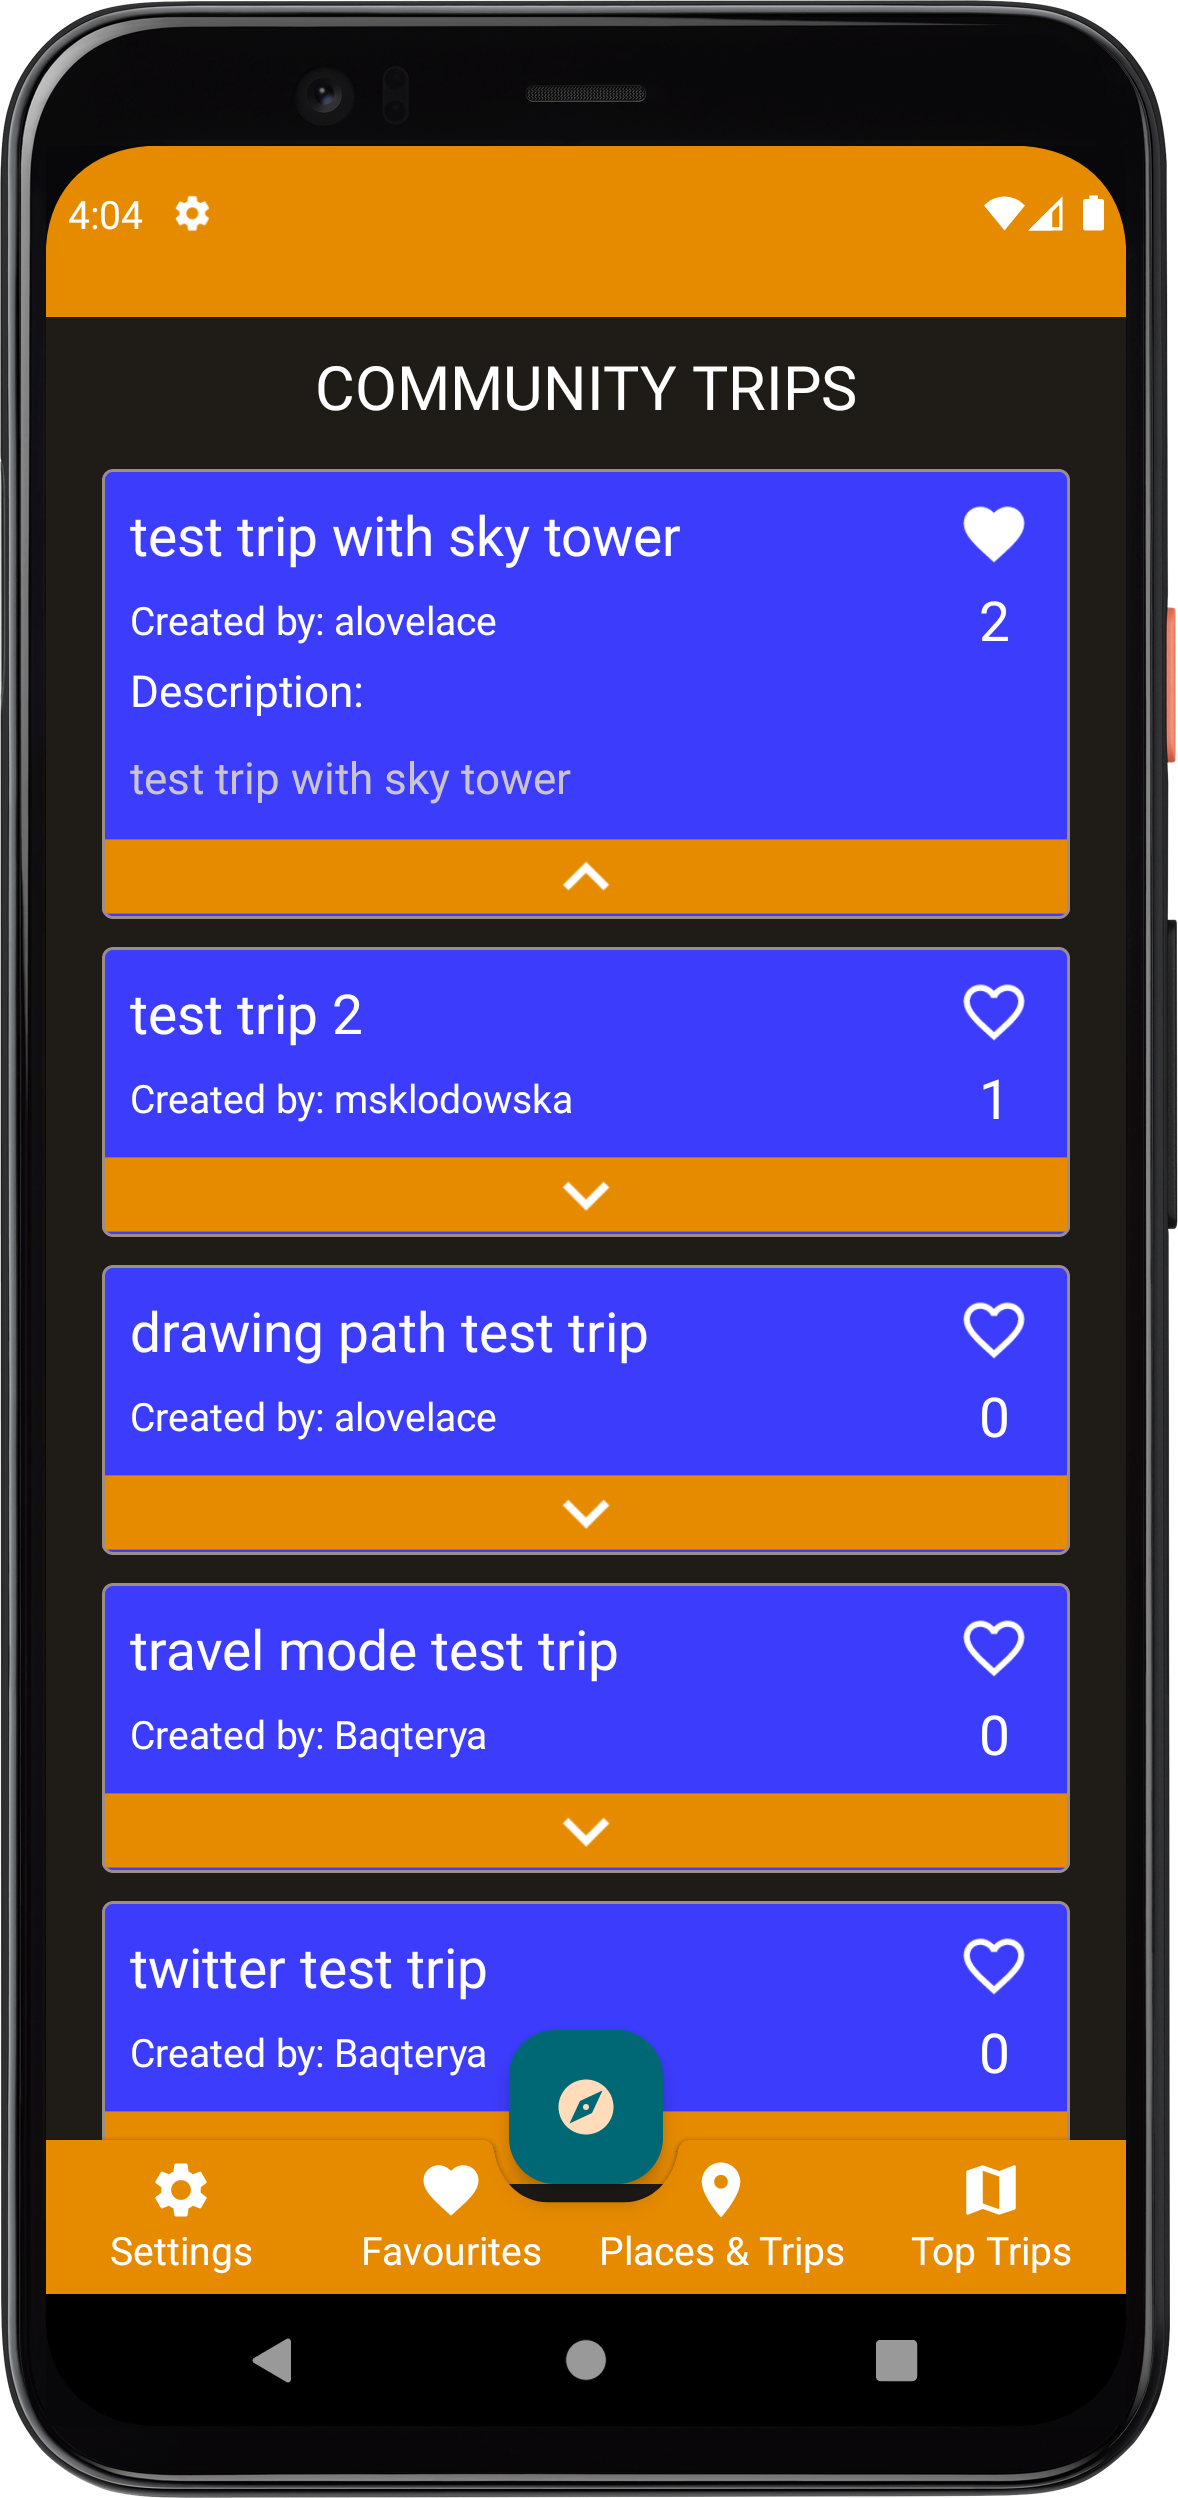
\includegraphics[scale=0.10]{src/app/top_trips.png}
            \caption{Ekran najpopularniejszych wycieczek.\label{top_trips}}
            \qquad
        \end{figure} 
        \vspace{1cm}